\chapter{Analyse du parcours universitaire des bacheliers (UCAD)}

\section{Introduction}

Ce chapitre s’intéresse à la trajectoire des bacheliers après leur admission à l’université, en particulier à l’Université Cheikh Anta Diop de Dakar (UCAD). 
L’objectif est d’évaluer l’impact des différentes réformes du baccalauréat sur l’orientation et la réussite universitaire des étudiants issus des séries concernées, en comparant leur parcours à celui des étudiants issus de séries dites « de référence ».

Dans un premier temps, nous analyserons l’évolution des effectifs inscrits à l’UCAD selon les séries de baccalauréat touchées par les réformes, afin d’identifier les changements éventuels dans les tendances d’accès à l’enseignement supérieur. 
Cette analyse descriptive permettra de repérer les effets potentiels des réformes sur les flux d’entrée à l’université.

Nous nous intéresserons ensuite aux établissements et départements universitaires dans lesquels ces bacheliers sont majoritairement orientés. 
Cela permettra de déterminer les filières de destination privilégiées selon la série d’origine, et d’évaluer dans quelle mesure les réformes ont influencé les choix ou opportunités d’orientation dans l’enseignement supérieur.

Enfin, une analyse longitudinale de type \textbf{suivi de cohorte} sera conduite pour examiner la progression académique des étudiants au fil du temps, en tenant compte de leurs taux de réussite, redoublement et abandon. 
Cette approche permettra non seulement d’observer les parcours individuels, mais aussi de \textbf{comparer les taux de diplômés des séries concernées par les réformes à ceux des séries de référence}, fournissant ainsi une base d’évaluation plus objective de l’efficacité des réformes en matière de réussite universitaire.

\newpage
\section{Évolution des inscriptions à l'UCAD}

\subsection{Les inscrits des série STEG et G}

\begin{figure}[ht]
\centering
\caption{Évolution des inscriptions à l'UCAD pour les séries STEG et G}
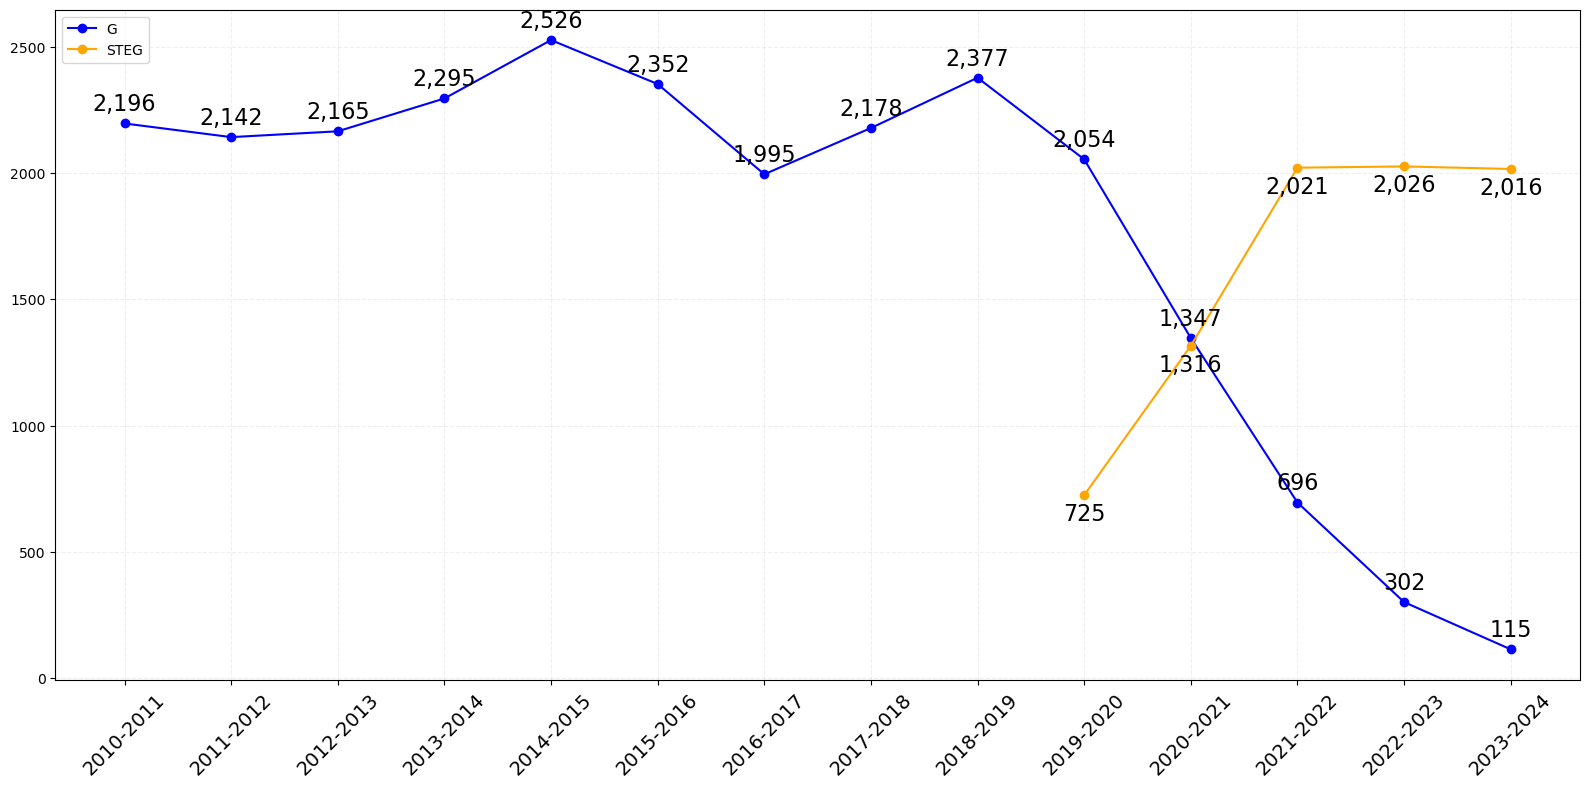
\includegraphics[width=1\textwidth]{figure/Inscrits_ucad_STEG.png}
\label{fig:inscrits_ucad_steg}
\end{figure}

La figure (Figure~\ref{fig:inscrits_ucad_steg}) illustre l'évolution des inscriptions à l'Université Cheikh Anta Diop (UCAD) pour les bacheliers issus des séries G et STEG, sur la période 2010-2011 à 2023-2024.

Jusqu'à l'année universitaire 2018-2019, seule la série G est représentée à l'UCAD, avec un nombre d'inscrits fluctuant autour de 2 000 à 2 500. Un pic est observé en 2014-2015 avec 2 526 inscrits. 
À partir de 2019-2020, la série STEG fait son apparition, avec 725 inscrits, marquant le début de la transition. Simultanément, les effectifs de la série G commencent à décliner fortement, passant de 2 054 en 2019-2020 à seulement 115 en 2023-2024. 
Ce déclin correspond à la suppression progressive de la série G au profit de la série STEG dans le système du baccalauréat.

Le croisement des courbes est particulièrement visible en 2020-2021, où le nombre d'inscrits en STEG (1 347) dépasse celui de la série G (1 316). 
Cette tendance se confirme les années suivantes, la série STEG affichant des effectifs croissants (2 021 en 2021-2022, 2 026 en 2022-2023, et 2 016 en 2023-2024), tandis que la série G continue sa chute. 
La série STEG maintient ainsi un volume d'inscriptions à l'UCAD comparable à celui que la série G connaissait avant sa suppression, démontrant une transition quantitativement réussie au niveau de l'entrée à l'université. 
Ce transfert des effectifs de la série G vers la série STEG à l'UCAD est un indicateur de l'efficacité de la réforme du baccalauréat dans l'orientation des étudiants vers la nouvelle filière.

\newpage
\subsection{Les inscrits des séries Arables et Franco-Arabes}

\subsubsection{Série LA et LAR}

\begin{figure}[ht]
\centering
\caption{Évolution des inscriptions à l'UCAD pour les séries LA et LAR}
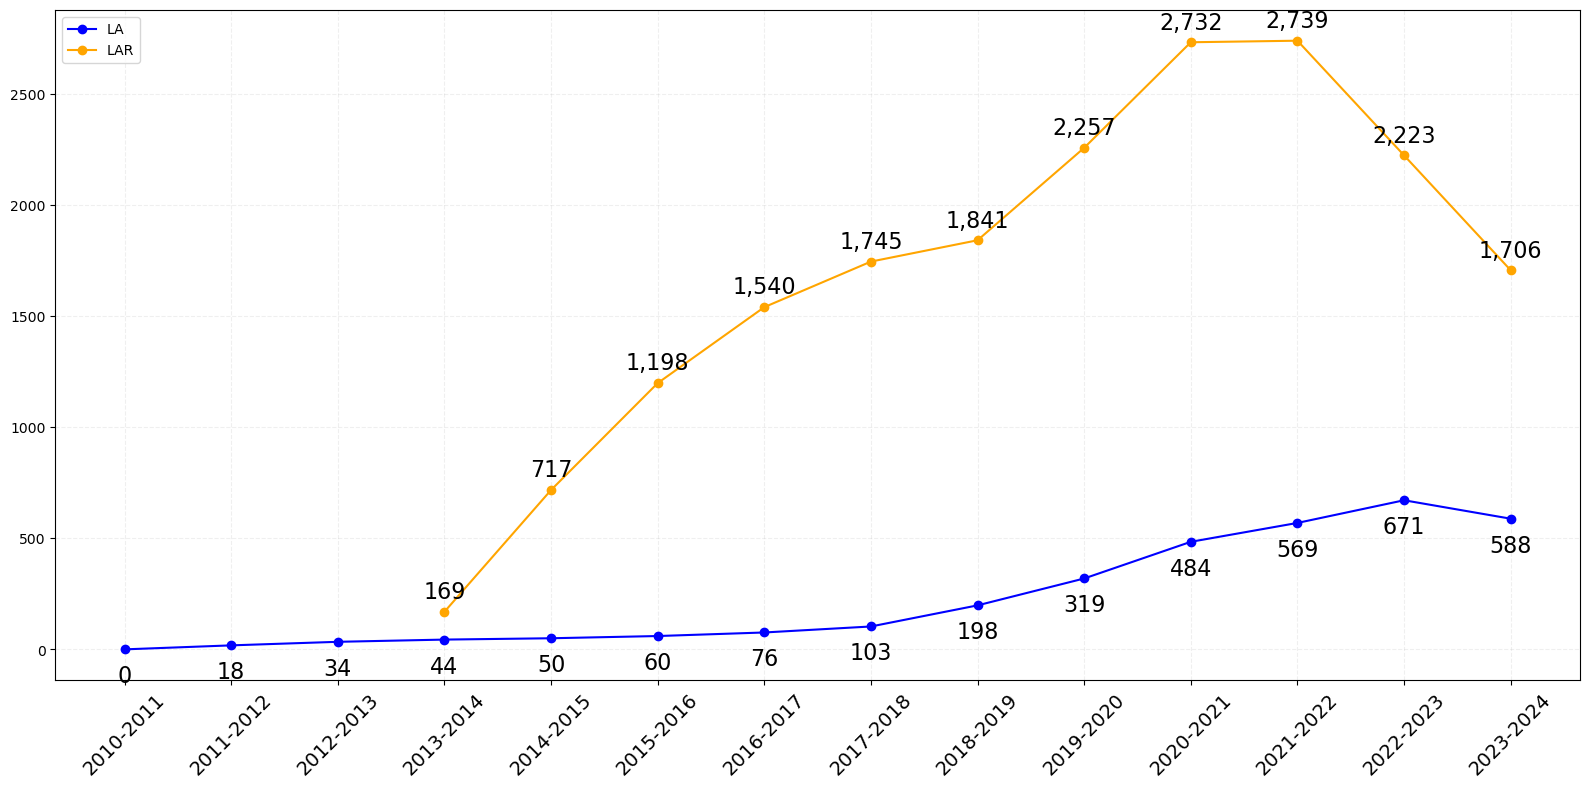
\includegraphics[width=1\textwidth]{figure/Inscrits_ucad_LA_LAR.png}
\label{fig:inscrits_ucad_la_lar}
\end{figure}

La figure (Figure~\ref{fig:inscrits_ucad_la_lar}) présente l'évolution des inscriptions à l'UCAD pour les bacheliers issus des séries Littératures Arabes (LA) et Littératures et Civilisations Arabes (L-AR) de 2010-2011 à 2023-2024.

La série LA, bien que présente depuis 2010-2011, a enregistré un nombre très faible d'inscrits à l'UCAD jusqu'en 2013-2014, oscillant entre 0 et 44. 
À partir de 2014-2015, le nombre d'inscrits en LA connaît une croissance progressive, passant de 50 à 671 en 2022-2023, avant de redescendre légèrement à 588 en 2023-2024.

La série L-AR, introduite à l'UCAD à partir de 2013-2014, a connu une croissance beaucoup plus rapide et significative. Elle débute avec 169 inscrits en 2013-2014 et grimpe rapidement pour atteindre un pic de 2 739 inscrits en 2021-2022. 
Bien qu'une légère diminution soit observée les années suivantes, avec 2 223 inscrits en 2022-2023 et 1 706 en 2023-2024, la série L-AR maintient un volume d'inscriptions considérablement plus élevé que la série LA. 
Ce phénomène s'aligne avec l'observation d'un transfert progressif des effectifs vers la série L-AR au niveau du baccalauréat lui-même, la série L-AR ayant été mise en place pour mieux encadrer et répondre à la demande sociale des filières arabes et franco-arabes. 

\newpage
\subsubsection{Série S2A et S1A}

\begin{figure}[ht]
\centering
\caption{Évolution des inscriptions à l'UCAD pour les séries S2A et S1A}
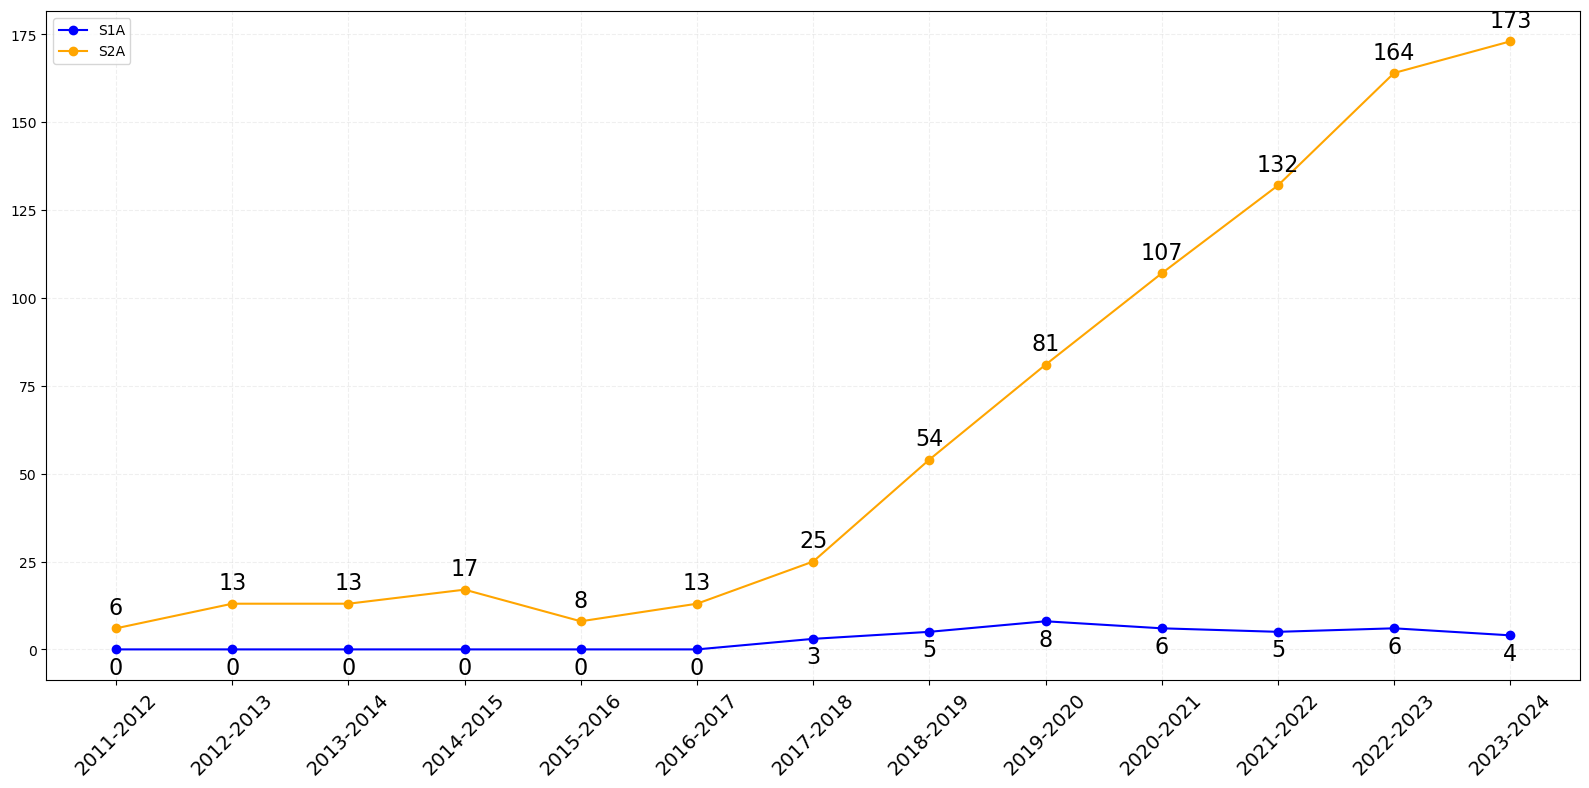
\includegraphics[width=1\textwidth]{figure/Inscrits_ucad_SA.png}
\label{fig:inscrits_ucad_sa}
\end{figure}

La figure (Figure~\ref{fig:inscrits_ucad_sa}) retrace l'évolution des inscriptions à l'UCAD pour les bacheliers des séries Sciences fondamentales (S1A) et Sciences appliquées (S2A) entre 2011-2012 et 2023-2024.

La série S1A, bien que présente, affiche un nombre d'inscrits extrêmement faible à l'UCAD tout au long de la période. Les effectifs oscillent entre 0 et 8 (atteint en 2019-2020), avec seulement 4 inscrits en 2023-2024. 
Cette quasi-absence d'inscriptions à l'université confirme le caractère très marginal de cette filière, qui déjà au niveau du baccalauréat, n'attire qu'un nombre dérisoire de candidats. 
Cela suggère que la série S1A ne débouche que sur très peu d'orientations universitaires à l'UCAD.

En revanche, la série S2A présente une dynamique d'inscriptions beaucoup plus significative. Après des débuts modestes entre 6 et 17 inscrits de 2011-2012 à 2015-2016, le nombre d'étudiants en S2A à l'UCAD connaît une croissance exponentielle. 
On passe de 25 inscrits en 2016-2017 à 107 en 2020-2021, pour atteindre un pic de 173 inscrits en 2023-2024. Cette forte augmentation des inscriptions en S2A à l'UCAD reflète une reconnaissance croissante de cette filière scientifique parmi les bacheliers arabes et franco-arabes, leur offrant des perspectives universitaires concrètes.

En somme, l'analyse des inscriptions à l'UCAD confirme les dynamiques observées au niveau du baccalauréat : la série S1A reste une filière confidentielle, tandis que la S2A gagne en importance et en attractivité pour les études supérieures, offrant ainsi une voie viable aux bacheliers issus de l'enseignement scientifique arabe et franco-arabe.

\newpage
\section{Répartition des Inscrits par Établissement et Département}

\subsection{Série STEG et G}

\textbf{Répartition par Établissements}

\begin{figure}[ht]
\centering
\caption{Top 5 des établissements avec le plus d'inscrits (G, 2018-2019)}
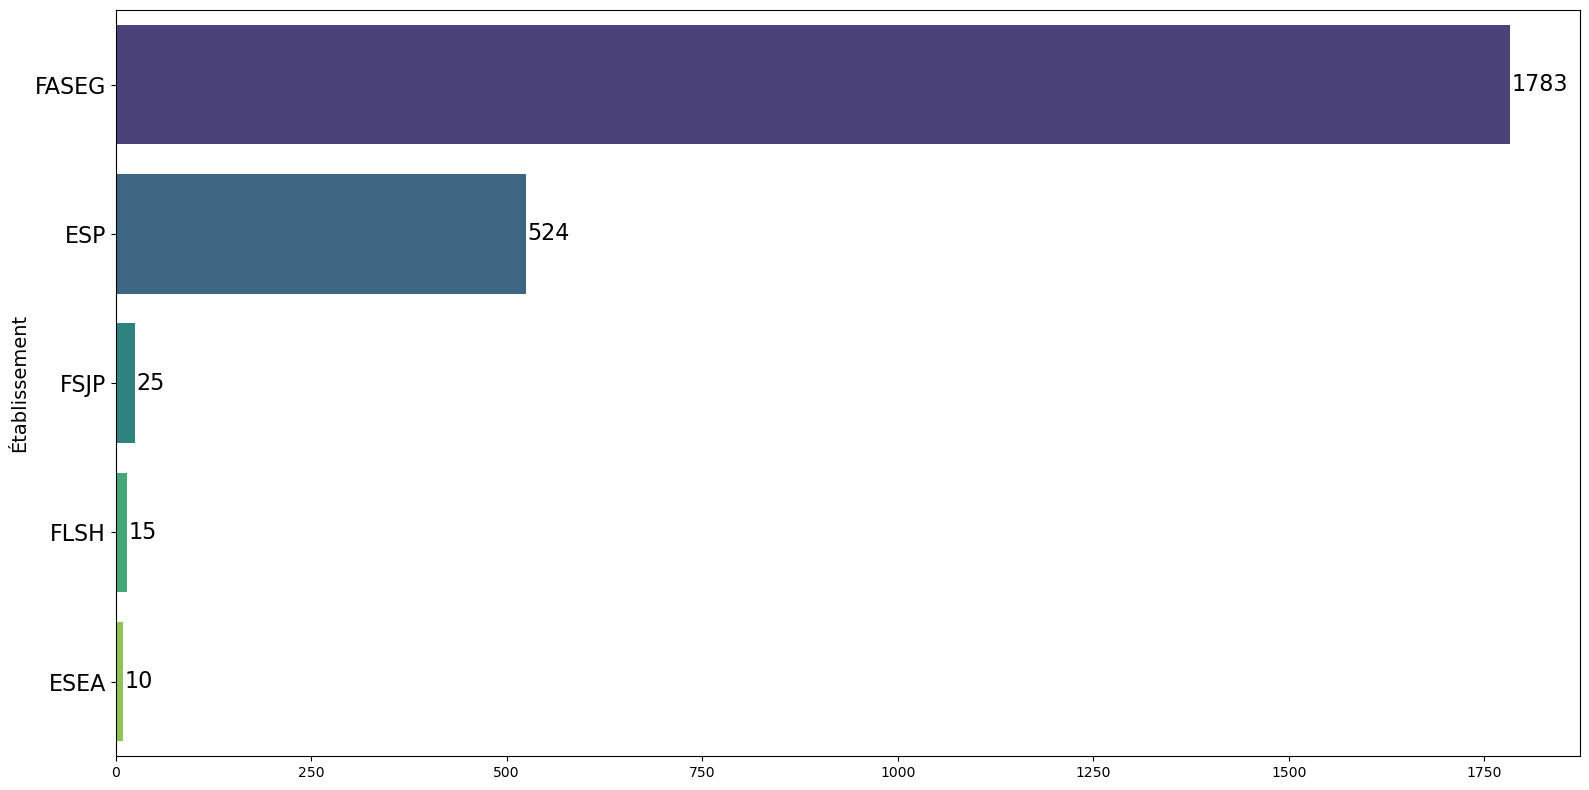
\includegraphics[width=0.85\textwidth]{figure/etab_G_2019.png}
\label{fig:etab_g_2019}
\end{figure}

La figure (Figure~\ref{fig:etab_g_2019}) présente la répartition des inscriptions des bacheliers G au sein des établissements de l'UCAD pour l'année universitaire 2018-2019.

Avant la réforme complète, en 2019, la Faculté des Sciences Économiques et de Gestion (FASEG) était déjà l'établissement accueillant la majorité des bacheliers de la série G, avec 1783 inscrits, suivie par l'École Supérieure Polytechnique (ESP) avec 524 inscrits. 

% \newpage
\begin{figure}[ht]
\centering
\caption{Top 5 des établissements avec le plus d'inscrits (STEG, 2023-2024)}
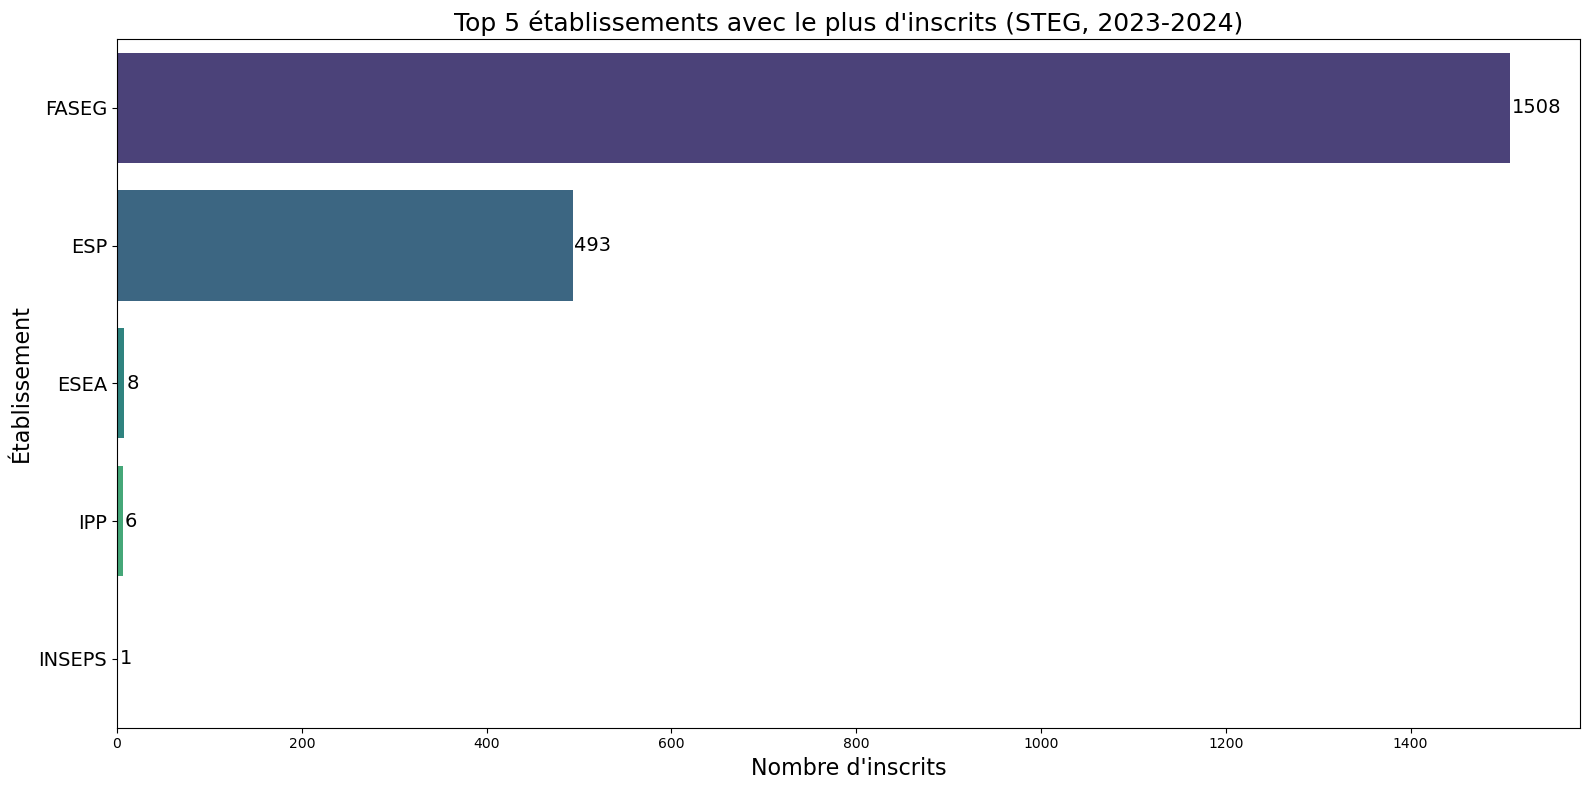
\includegraphics[width=0.85\textwidth]{figure/etab_STEG_2024.png}
\label{fig:etab_steg_2024}
\end{figure}

La figure (Figure~\ref{fig:etab_steg_2024}) présente la répartition des inscriptions des bacheliers STEG au sein des établissements de l'UCAD pour l'année universitaire 2023-2024.

Pour l'année universitaire 2023-2024, après la transformation de la série G en STEG, la FASEG continue de dominer très largement les inscriptions des bacheliers STEG à l'UCAD, accueillant 1508 étudiants. 
L'École Supérieure Polytechnique (ESP) maintient sa deuxième position avec 493 inscrits. Ces chiffres confirment que, malgré le changement de dénomination et d'orientation pédagogique, la FASEG demeure la principale destination pour les bacheliers de cette filière, en raison de la nature économique et de gestion de la série STEG. 

% \newpage
\textbf{Répartition par Départements}

\begin{figure}[ht]
\centering
\caption{Top 5 des départements avec le plus d'inscrits (G, 2018-2019)}
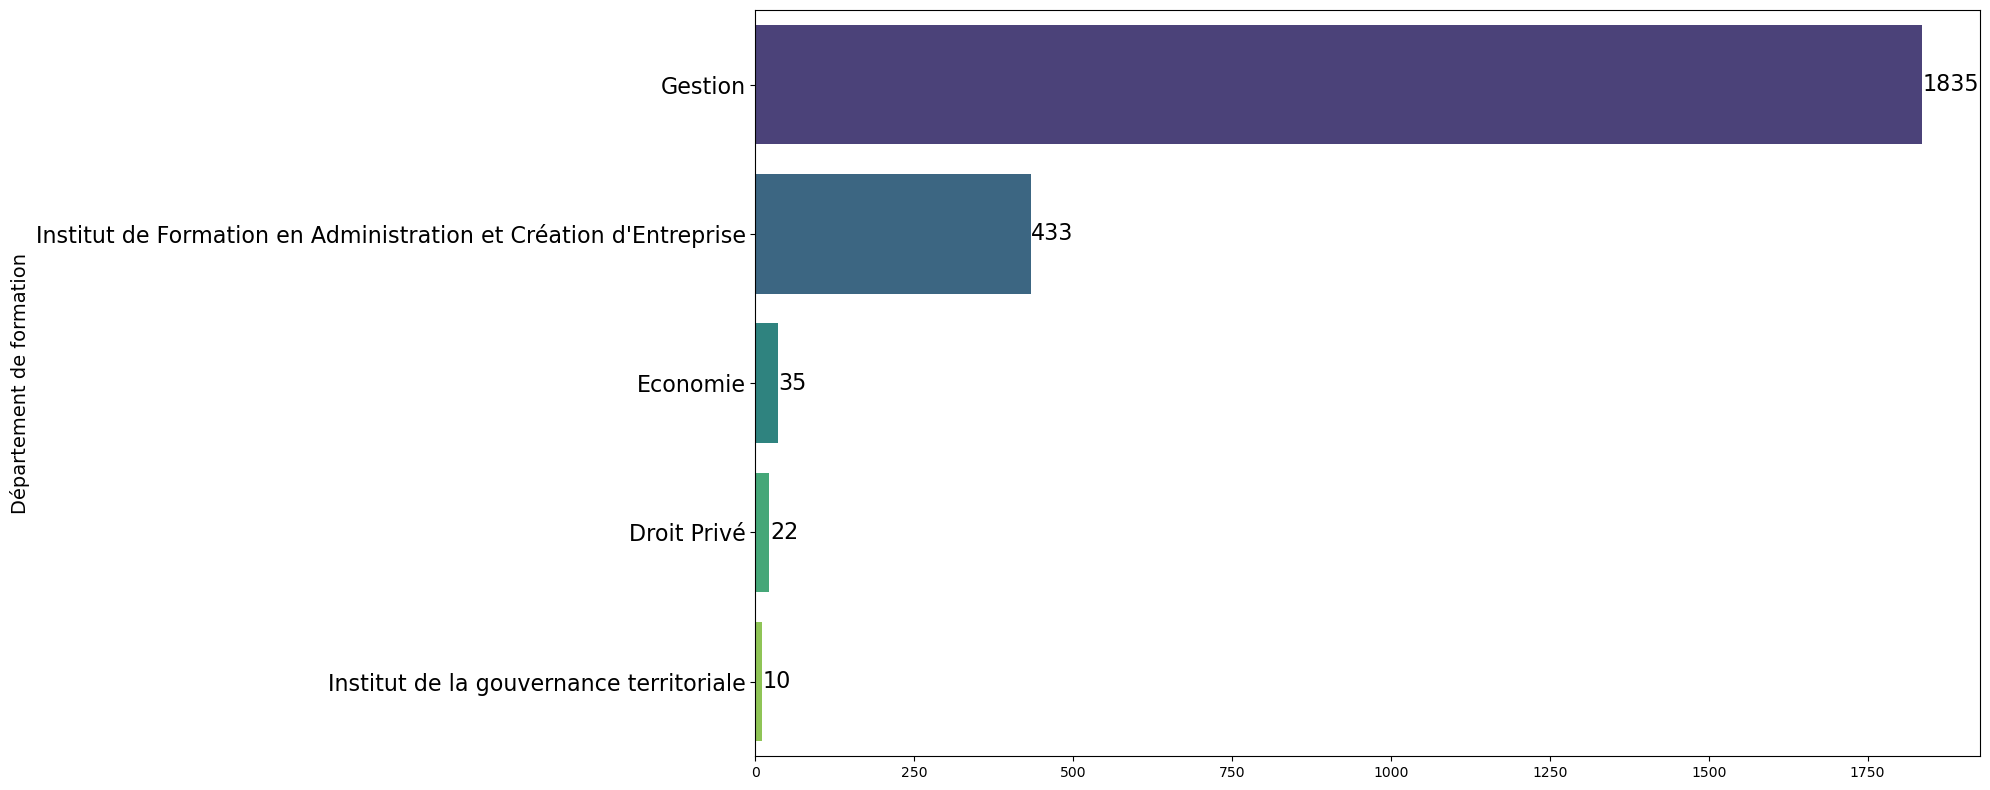
\includegraphics[width=0.85\textwidth]{figure/dep_G_2019.png}
\label{fig:dep_g_2019}
\end{figure}

La figure (Figure~\ref{fig:dep_g_2019}) illustre la répartition des inscrits G par département de formation à l'UCAD pour l'année universitaire 2018-2019.

En 2019, le département de Gestion concentrait la grande majorité des inscrits de la série G, avec 1835 étudiants, suivi par l'Institut de Formation en Administration et Création d'Entreprise avec 433 inscrits. Le département d'Économie comptait 35 inscrits.

% Le département de Gestion se positionne très largement en tête, avec 1 623 inscrits. Cette dominance est logique et attendue, étant donné l'orientation principale de la série G vers les sciences et techniques de gestion. 

\begin{figure}[ht]
\centering
\caption{Top 5 des départements avec le plus d'inscrits (STEG, 2023-2024)}
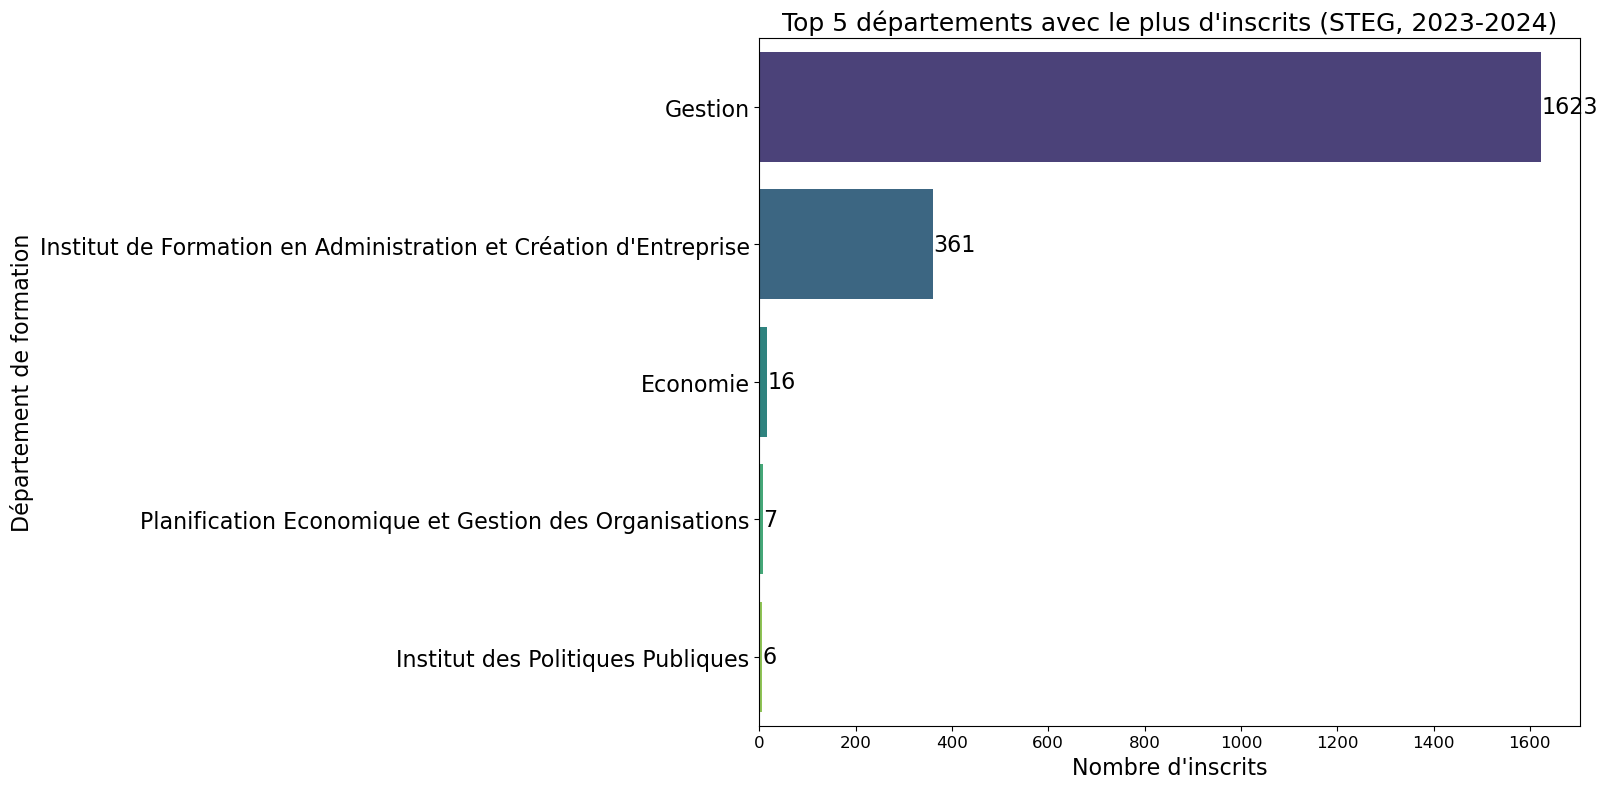
\includegraphics[width=0.85\textwidth]{figure/dep_STEG_2024.png}
\label{fig:dep_steg_2024}
\end{figure}

La figure (Figure~\ref{fig:dep_steg_2024}) illustre la répartition des inscrits STEG par département de formation à l'UCAD pour l'année universitaire 2023-2024.

Pour l'année universitaire 2023-2024, le département de Gestion conserve sa position dominante pour les inscrits de la série STEG, avec 1623 inscrits. L'Institut de Formation en Administration et Création d'Entreprise suit avec 361 inscrits. 
Le département d'Économie compte 16 inscrits. Cette répartition des inscrits par département, avant et après la réforme, confirme la forte vocation de cette série pour les études en gestion, avec un intérêt secondaire pour l'entrepreneuriat, et une présence marginale dans les autres branches de l'économie. 

% \newpage
\subsection{Série Arabes et Franco-Arabes}

\subsubsection{Série LA}

\textbf{Établissements}

\begin{figure}[ht]
\centering
\caption{Top 5 des établissements avec le plus d'inscrits (LA, 2023-2024)}
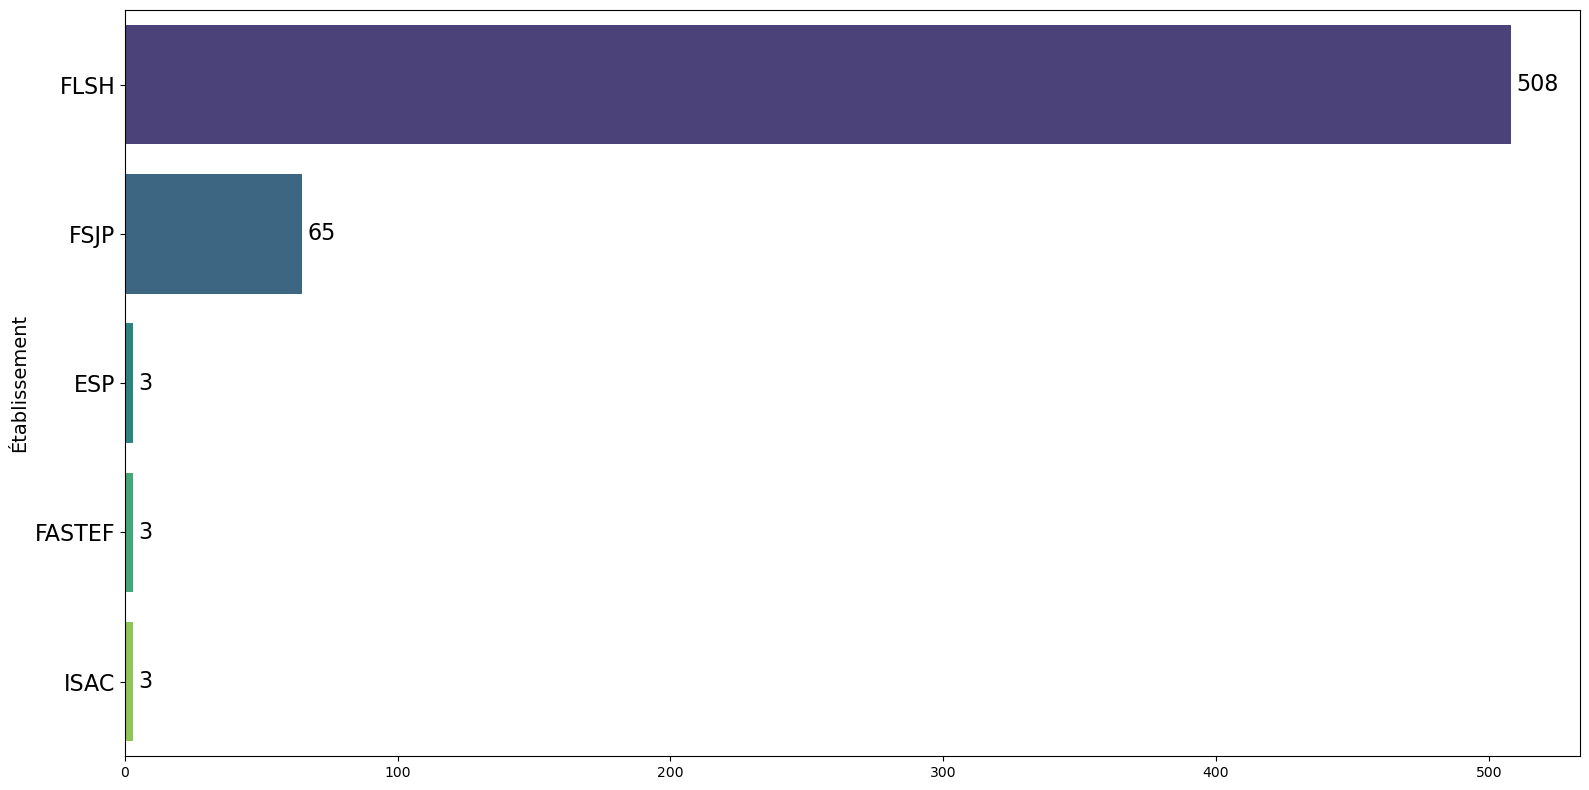
\includegraphics[width=0.85\textwidth]{figure/etab_LA_2024.png}
\label{fig:etab_la_2024}
\end{figure}

La figure (Figure~\ref{fig:etab_la_2024}) montre la répartition des inscrits de la série LA par établissement à l'UCAD pour l'année universitaire 2023-2024.

La Faculté des Lettres et Sciences Humaines (FLSH) est l'établissement qui accueille de loin le plus grand nombre de bacheliers LA, avec 508 inscrits. 
Cette prédominance est entièrement cohérente avec la nature littéraire de la série LA.

La Faculté des Sciences Juridiques et Politiques (FSJP) arrive en deuxième position avec 65 inscrits. Bien que significativement moins importante que la FLSH, la présence de bacheliers LA dans cette faculté peut s'expliquer par un intérêt pour le droit islamique.

\textbf{Départements}

\begin{figure}[ht]
\centering
\caption{Top 5 des départements avec le plus d'inscrits (LA, 2023-2024)}
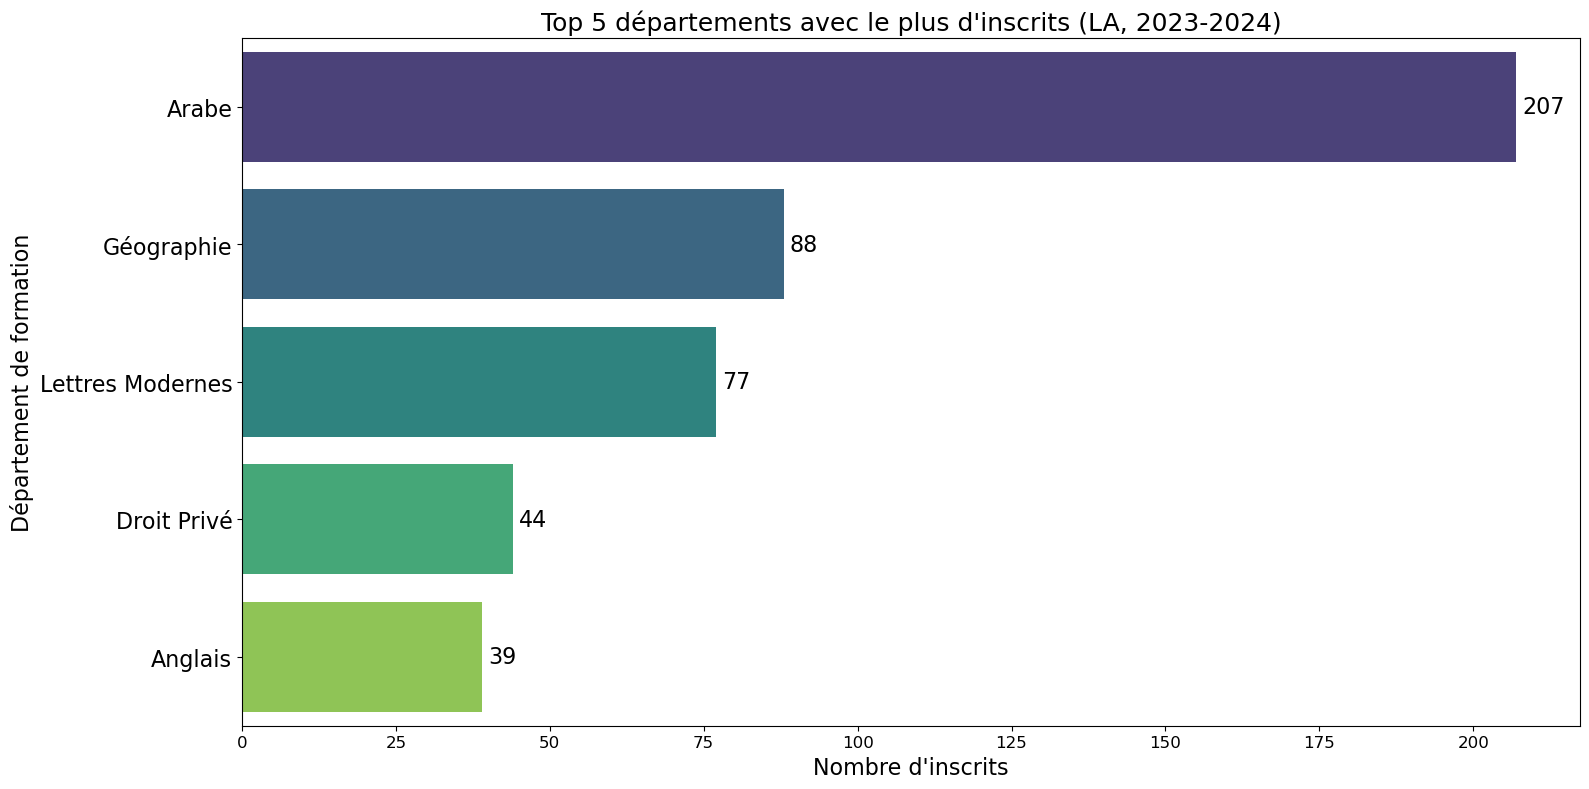
\includegraphics[width=0.85\textwidth]{figure/dep_LA_2024.png}
\label{fig:dep_la_2024}
\end{figure}

La figure (Figure~\ref{fig:dep_la_2024}) présente la répartition des inscrits de la série LA par département de formation à l'UCAD pour l'année universitaire 2023-2024.

Le département d'Arabe domine avec 207 bacheliers LA, ce qui est attendu pour cette série littéraire axée sur la langue arabe
Cependant, d’autres départements comme la Géographie (88), les Lettres Modernes (77), le Droit Privé (44) et l’Anglais (39) attirent aussi des bacheliers LA

Cette dispersion s’explique par le caractère franco-arabe de la série LA, qui \textbf{offre plus de flexibilité que la série LAR}, permettant aux étudiants de s’orienter vers un éventail plus large.

\subsubsection{Série LAR}

\textbf{Établissements}

\begin{figure}[ht]
\centering
\caption{Top 5 des établissements avec le plus d'inscrits (LAR, 2023-2024)}
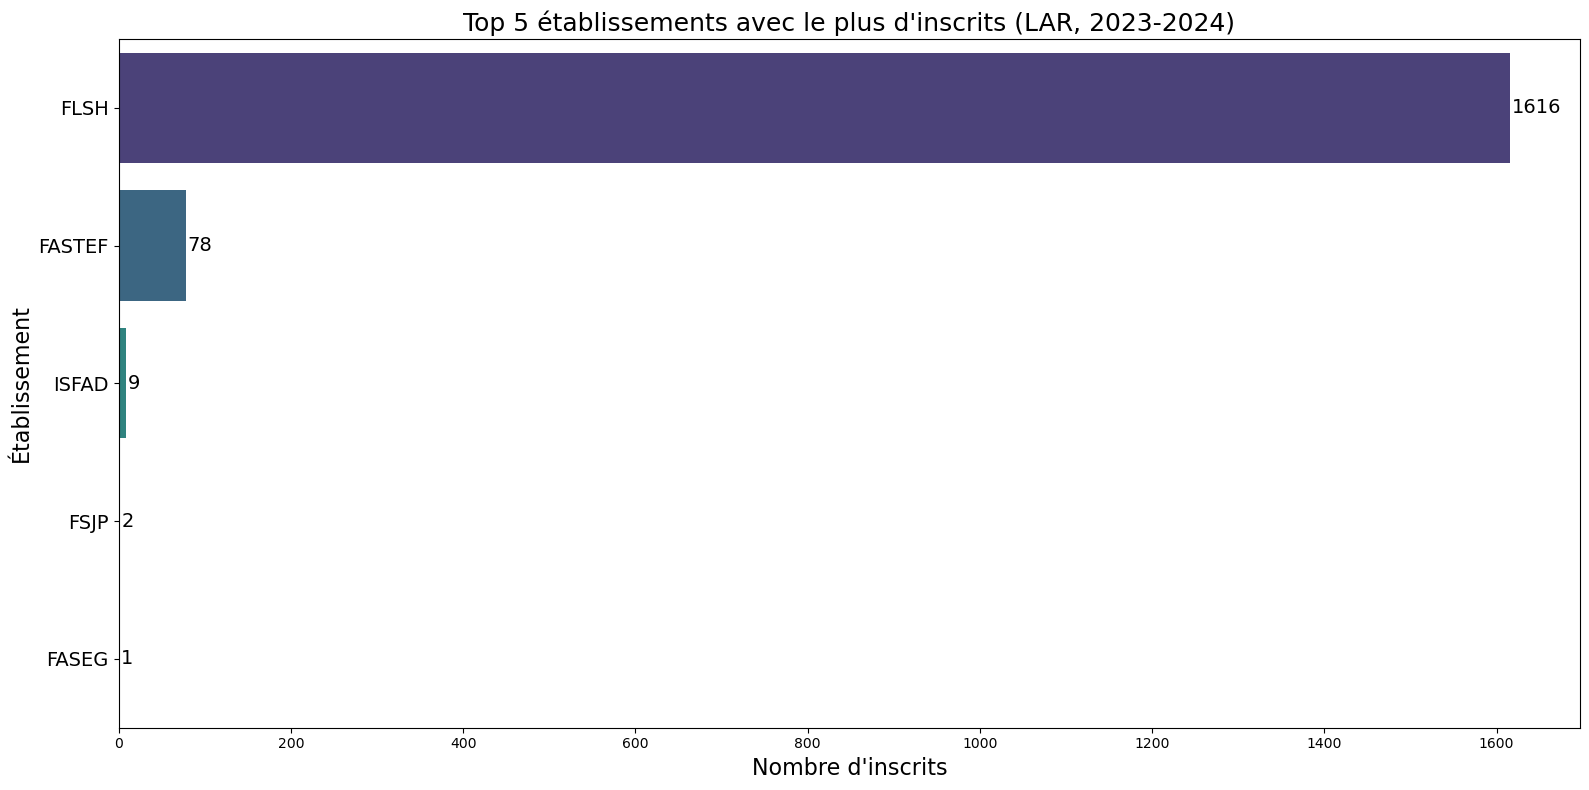
\includegraphics[width=0.85\textwidth]{figure/etab_LAR_2024.png}
\label{fig:etab_lar_2024}
\end{figure}

La figure (Figure~\ref{fig:etab_lar_2024}) illustre la répartition des inscrits de la série LAR par établissement à l'UCAD pour l'année universitaire 2023-2024.

Comme pour la série LA, la Faculté des Lettres et Sciences Humaines (FLSH) est l’établissement le plus plébiscité par les bacheliers LAR, avec un total massif de 1 616 inscrits. 
Cette écrasante majorité confirme le rôle central de la FLSH dans la formation en langue, littérature et civilisation arabes, faisant de cette faculté la destination naturelle et presque exclusive des bacheliers issus de cette série.

En deuxième position, la FASTEF accueille 78 inscrits. Cette orientation s'explique par les débouchés dans l’enseignement, en particulier pour les matières liées à la langue arabe ou à l’éducation islamique, domaines en cohérence avec la formation reçue dans la série LAR.

À l’inverse, la Faculté des Sciences Juridiques et Politiques (FSJP) ne compte que 2 inscrits LAR, contre 65 pour la série LA. 
Cette faible représentation s’explique très probablement par \textbf{une contrainte linguistique importante} : 
les enseignements à la FSJP se déroulant majoritairement en français, les bacheliers LAR, dont la formation est exclusivement en arabe, peuvent être freinés dans leur orientation vers des filières francophones.

\textbf{Départements}

\begin{figure}[ht]
\centering
\caption{Top 5 des départements avec le plus d'inscrits (LAR, 2023-2024)}
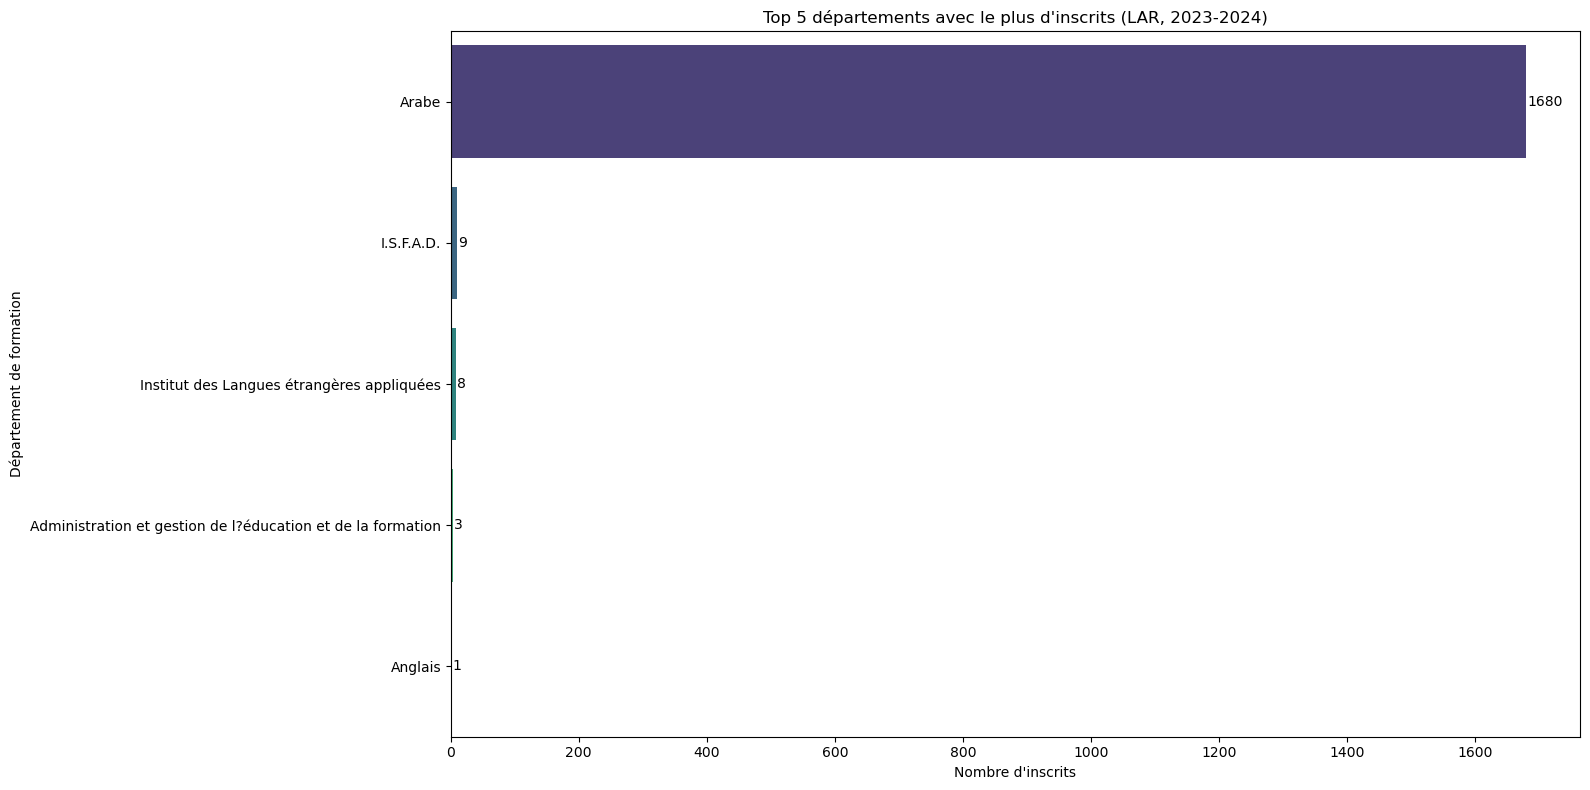
\includegraphics[width=0.85\textwidth]{figure/dep_LAR_2024.png}
\label{fig:dep_lar_2024}
\end{figure}

La figure (Figure~\ref{fig:dep_lar_2024}) détaille la répartition des inscrits de la série LAR par département de formation à l'UCAD pour l'année universitaire 2023-2024.

Le département d’Arabe domine de manière écrasante avec 1 680 inscrits, concentrant ainsi presque la totalité des bacheliers LAR. 
Cette prépondérance est tout à fait attendue, la série LAR (Littératures et Civilisations Arabes) étant spécifiquement conçue pour préparer les étudiants à des études approfondies en langue, littérature et culture arabes. 
Le département d’Arabe représente donc la destination la plus logique, naturelle et cohérente pour ces profils.

% En conclusion, l’orientation des bacheliers LAR est quasiment exclusive vers le département d’Arabe, traduisant une spécialisation universitaire marquée, en parfaite continuité avec leur formation secondaire.

\subsubsection{Série S2A}

\textbf{Établissements}

\begin{figure}[ht]
\centering
\caption{Top 5 des établissements avec le plus d'inscrits (S2A, 2023-2024)}
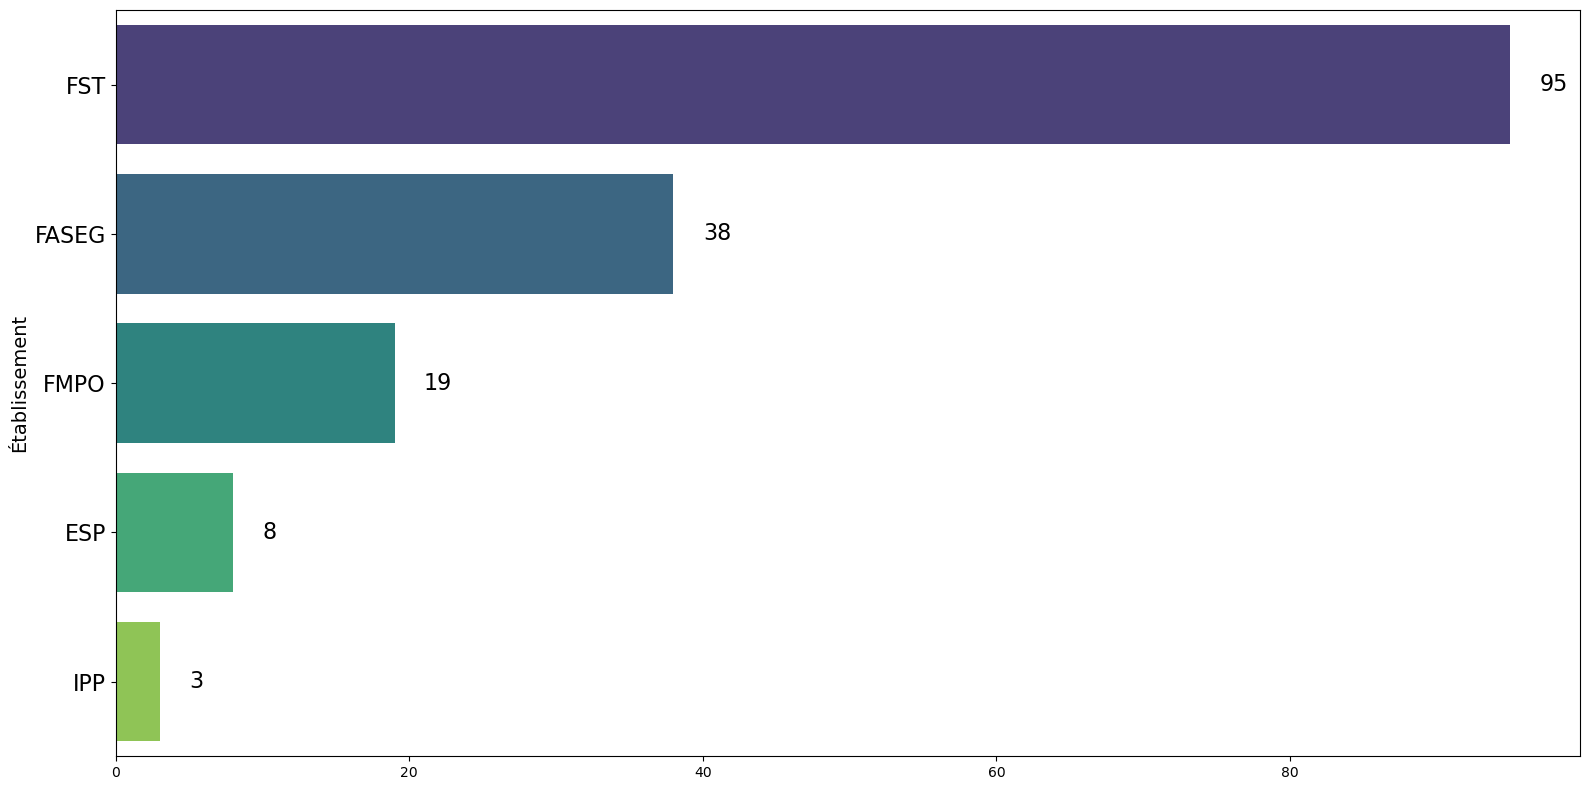
\includegraphics[width=0.85\textwidth]{figure/etab_S2A_2024.png}
\label{fig:etab_s2a_2024}
\end{figure}

La figure (Figure~\ref{fig:etab_s2a_2024}) présente la répartition des inscrits de la série S2A par établissement à l'UCAD pour l'année universitaire 2023-2024.

La FST domine avec 95 inscrits, reflet de l’orientation scientifique de la série S2A. 
D’autres établissements accueillent aussi ces étudiants, notamment la FASEG (38), la FMPO (19), ainsi que plus modestement l’ESP et l’IPP. Cette répartition illustre la polyvalence et l’adaptabilité des diplômés S2A, qui s’intègrent dans des filières variées allant des sciences à l’économie, la santé ou l’ingénierie.

\textbf{Départements}

\begin{figure}[ht]
\centering
\caption{Top 5 des départements avec le plus d'inscrits (S2A, 2023-2024)}
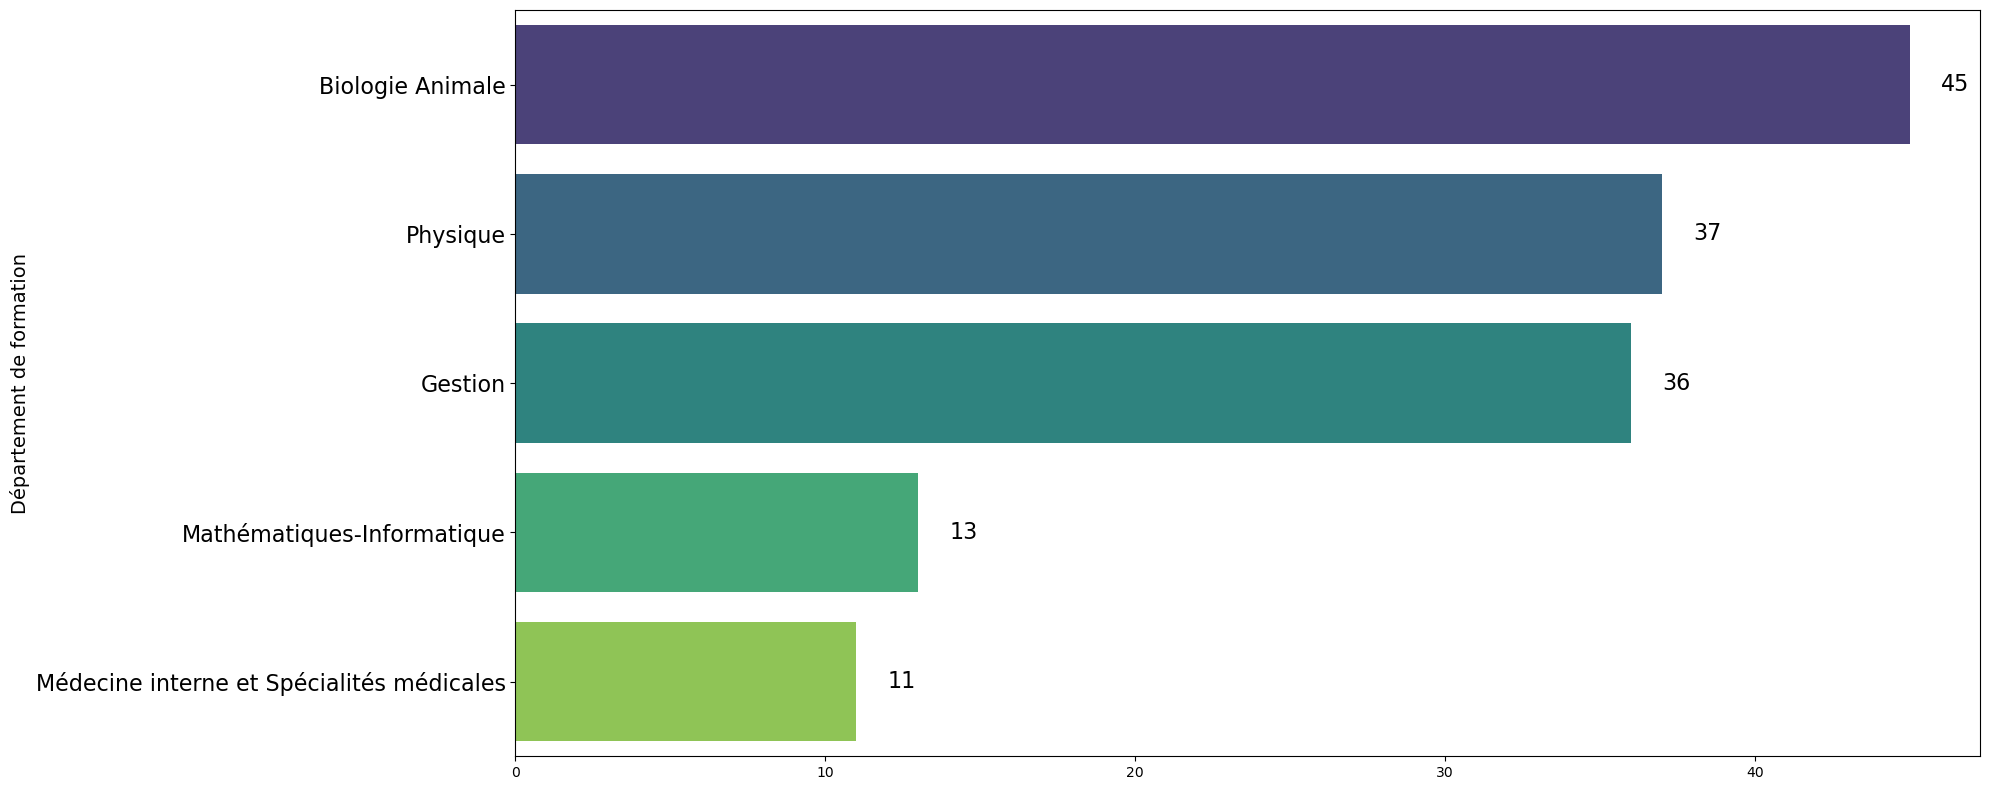
\includegraphics[width=0.85\textwidth]{figure/dep_S2A_2024.png}
\label{fig:dep_s2a_2024}
\end{figure}

La figure (Figure~\ref{fig:dep_s2a_2024}) détaille la répartition des inscrits de la série S2A par département de formation à l'UCAD pour l'année universitaire 2023-2024.

Le département de Biologie Animale accueille le plus grand nombre de bacheliers S2A (45 inscrits), reflétant leur intérêt pour les sciences du vivant. 
Les départements de Mathématiques-Informatique (13) et de Médecine (11) enregistrent des effectifs plus modestes, montrant une ouverture vers des filières techniques et médicales. 
Cette diversité souligne la capacité des bacheliers S2A à s’intégrer dans des parcours variés grâce à leur formation polyvalente.

\subsubsection{Série S1A}

\textbf{Établissements}

\begin{figure}[ht]
\centering
\caption{Top 5 des établissements avec le plus d'inscrits (S1A, 2023-2024)}
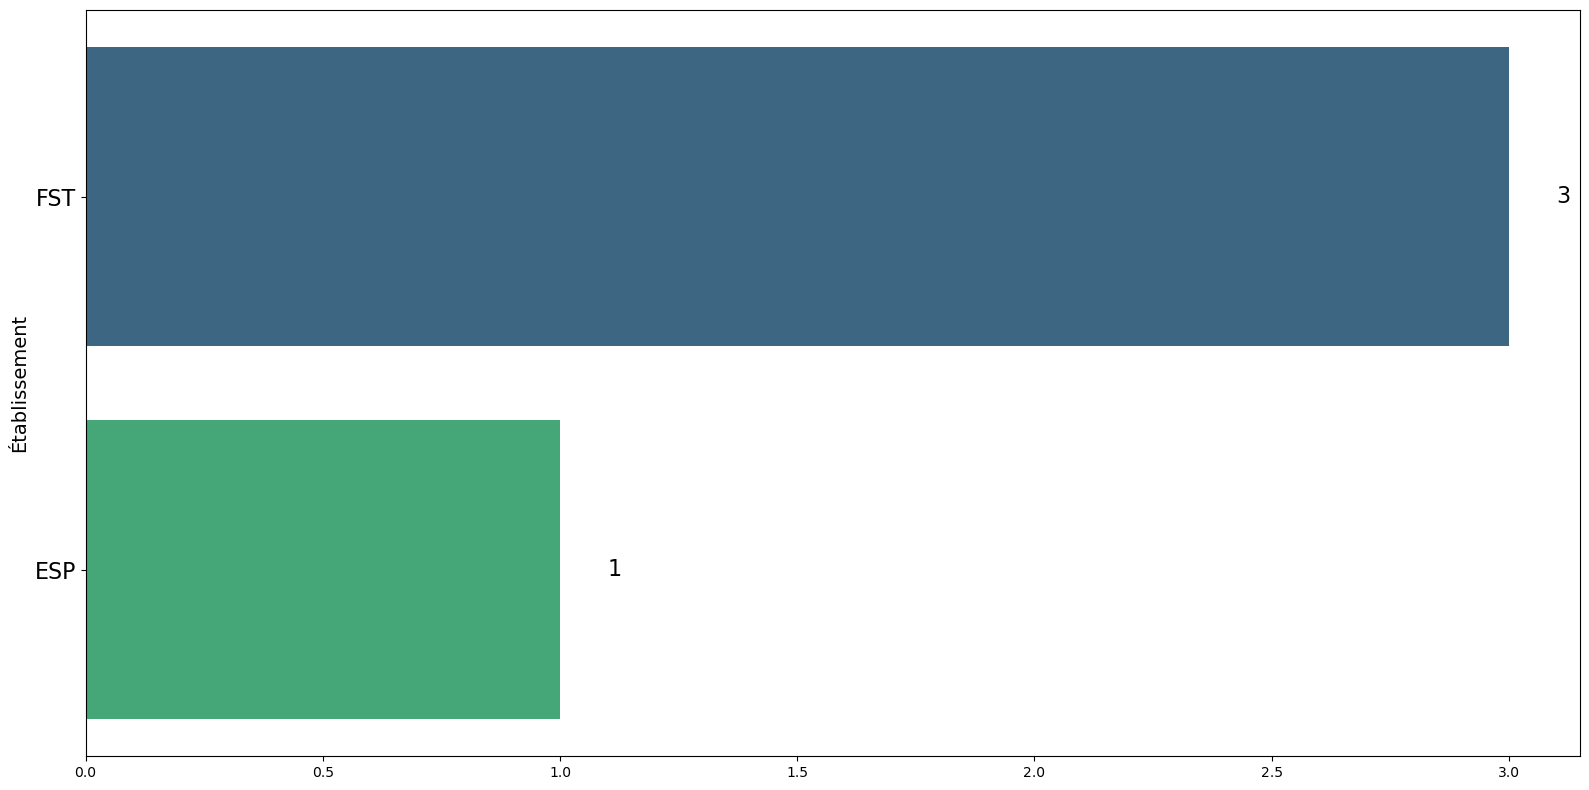
\includegraphics[width=0.8\textwidth]{figure/etab_S1A_2024.png}
\label{fig:etab_s1a_2024}
\end{figure}

La Figure \ref{fig:etab_s1a_2024} présente la répartition des inscrits de la série S1A par établissement à l'UCAD pour l'année universitaire 2023-2024.

La Faculté des Sciences et Technologies (FST) est la principale destination avec 3 inscrits, ce qui correspond à la nature fondamentale de la série S1A. 
L’École Supérieure Polytechnique (ESP) accueille un seul inscrit, reflétant un intérêt marginal pour les formations techniques.

Cependant, le très faible nombre d’inscrits dans ces établissements souligne la rareté de cette série à l’UCAD. 
Ces données limitées ne permettent pas de tirer de conclusions robustes sur les choix d’orientation des bacheliers S1A.

\newpage
\textbf{Départements}

\begin{figure}[ht]
\centering
\caption{Top 5 des départements avec le plus d'inscrits (S1A, 2023-2024)}
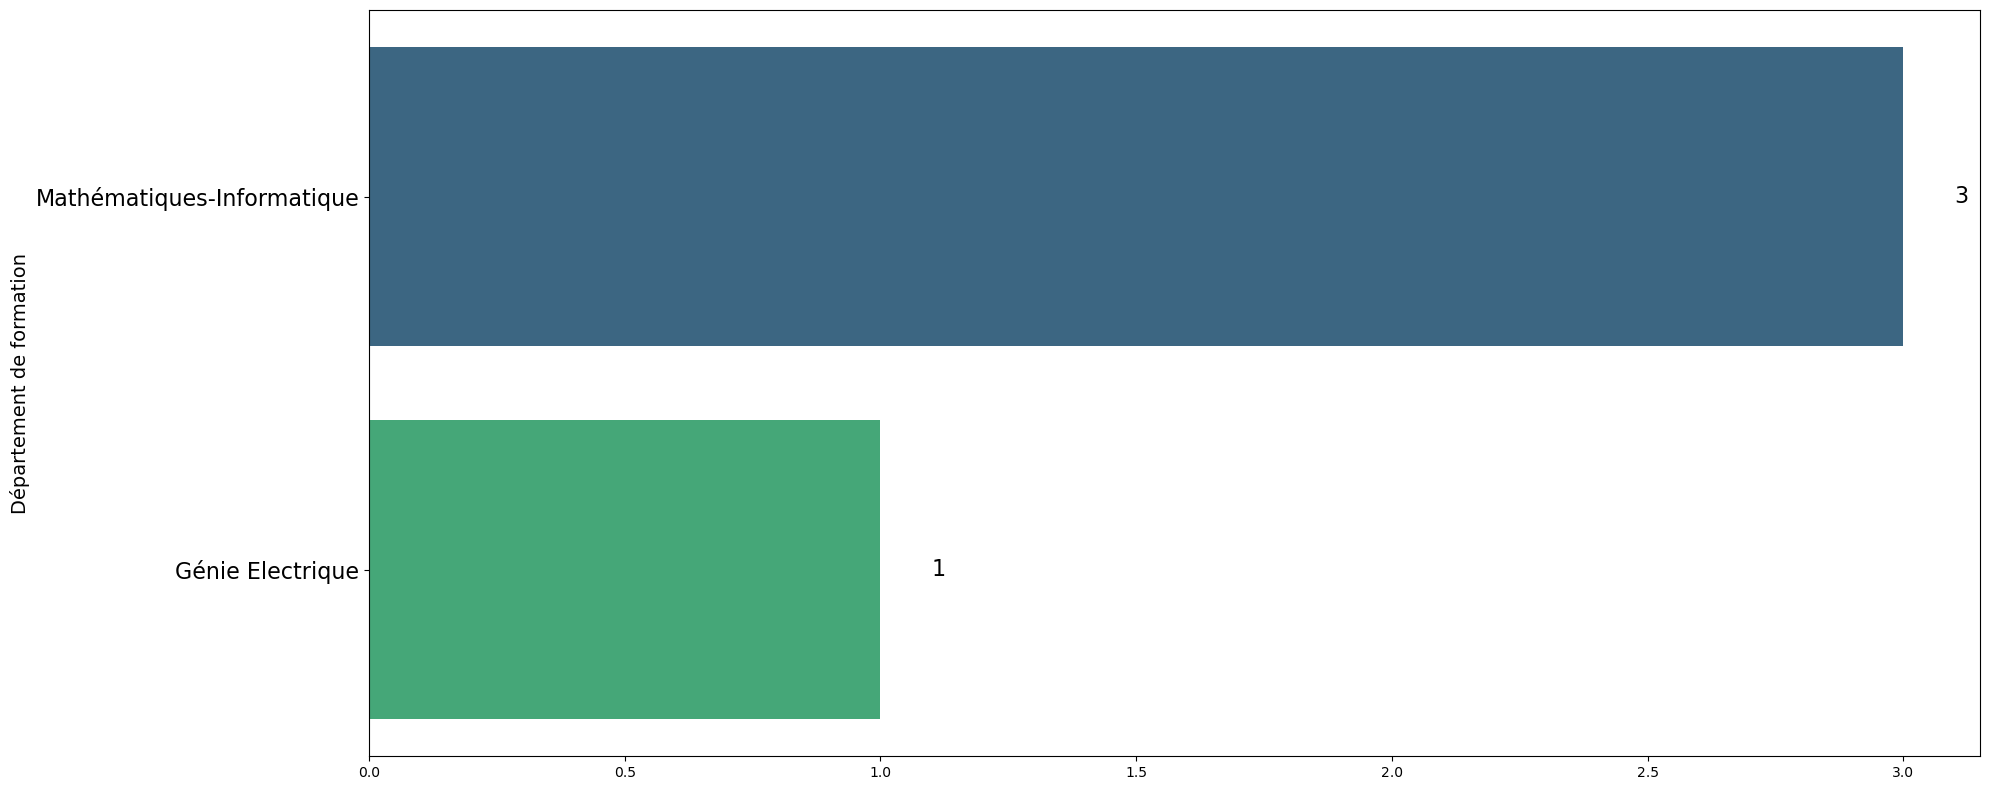
\includegraphics[width=0.8\textwidth]{figure/dep_S1A_2024.png}
\label{fig:dep_s1a_2024}
\end{figure}

La Figure \ref{fig:dep_s1a_2024} illustre la répartition des inscrits de la série S1A par département de formation à l'UCAD pour l'année universitaire 2023-2024.

Le département de Mathématiques-Informatique compte 3 inscrits, ce qui correspond bien au profil scientifique fondamental de la série S1A. Le Génie Électrique accueille 1 étudiant, reflétant un intérêt pour des applications techniques. 
Ces effectifs limités confirment la faible présence des bacheliers S1A à l’UCAD, qui restent néanmoins orientés vers des filières scientifiques et d’ingénierie spécialisées.

\newpage
\section{Analyse du parcours universitaire des bacheliers (suivi des cohortes)}

\subsection{Série Arabes et Franco-Arabes}
\subsubsection{cohorte 2018(LA)}

\begin{figure}[ht]
    \centering
    \caption{Graphe suivi de la cohorte 2018 (LA)}
    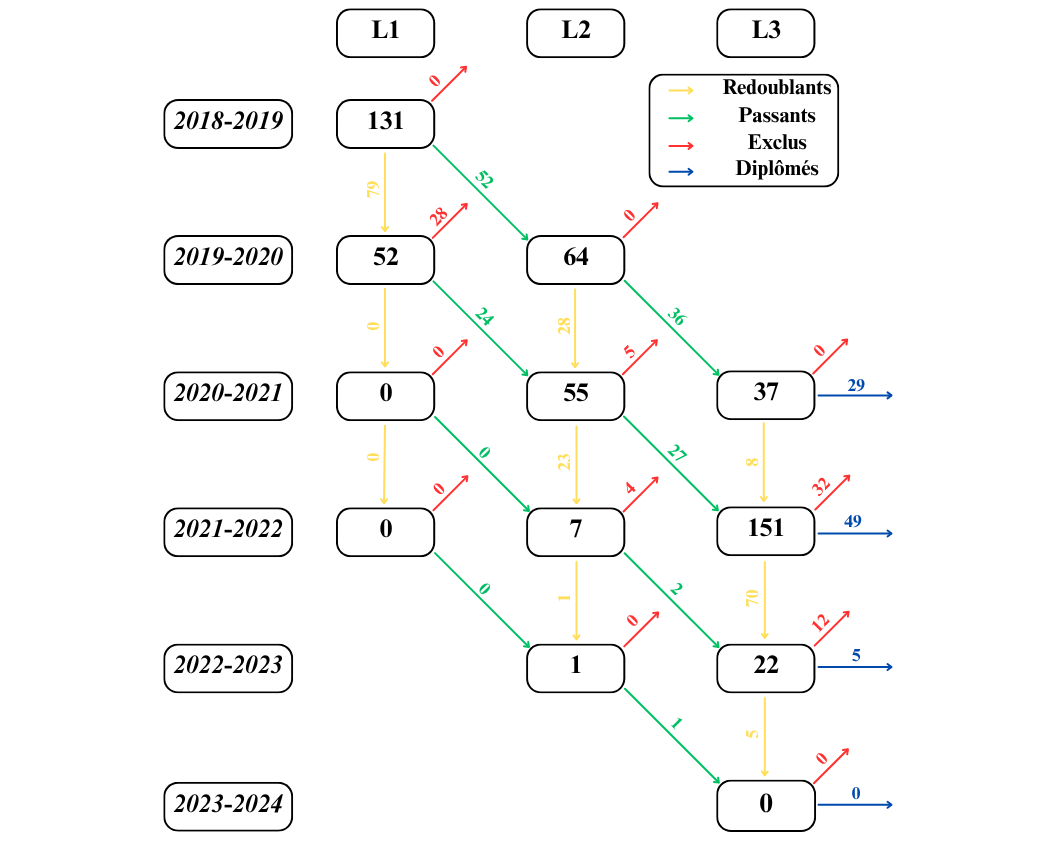
\includegraphics[width=1\textwidth]{figure/LA_2018.png}
    \label{fig:cohorte_la_2018}
\end{figure}

La figure (Figure~\ref{fig:cohorte_la_2018}) montre le suivi de la cohorte 2018 de la série LA.
\begin{itemize}
    \item Après 3 ans (en 2020-2021), sur les 131 étudiants initiaux en L1 en 2018-2019, 29 ont obtenu leur diplôme, soit un taux de diplomation d'environ 22.14\%.
    \item Après 4 ans (en 2021-2022), 49 étudiants supplémentaires ont été diplômés, portant le total à 78 diplômés, soit un taux cumulé d'environ 59.54\%.
    \item Après 5 ans (en 2022-2023), 5 étudiants supplémentaires ont été diplômés, portant le total à 83 diplômés, soit un taux cumulé d'environ 63.36\%.
    \item Après 6 ans (en 2023-2024), aucun étudiant supplémentaire n'a été diplômé, le total restant à 83 diplômés, soit un taux cumulé d'environ 63.36\%.
\end{itemize}

\subsubsection{cohorte 2018(LAR)}

\begin{figure}[ht]
    \centering
    \caption{Graphe suivi de la cohorte 2018 (LAR)}
    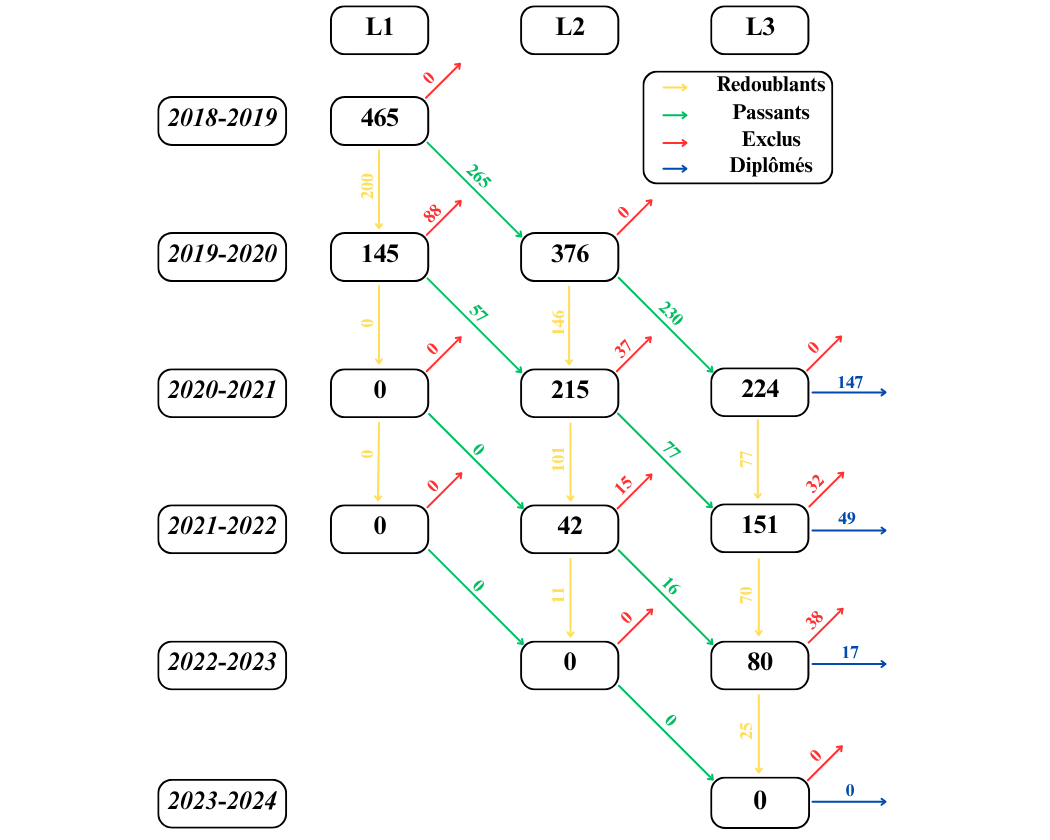
\includegraphics[width=1\textwidth]{figure/LAR_2018.png}
    \label{fig:cohorte_lar_2018}
\end{figure}

La figure \ref{fig:cohorte_lar_2018} présente le suivi de la cohorte 2018 de la série LAR.
\begin{itemize}
    \item Après 3 ans (en 2020-2021), sur les 465 étudiants initiaux en L1 en 2018-2019, 147 ont obtenu leur diplôme, soit un taux de diplomation d'environ 31.61\%.
    \item Après 4 ans (en 2021-2022), 49 étudiants supplémentaires ont été diplômés, portant le total à 196 diplômés, soit un taux cumulé d'environ 42.15\%.
    \item Après 5 ans (en 2022-2023), 17 étudiants supplémentaires ont été diplômés, portant le total à 213 diplômés, soit un taux cumulé d'environ 45.81\%.
    \item Après 6 ans (en 2023-2024), aucun étudiant supplémentaire n'a été diplômé, le total restant à 213 diplômés, soit un taux cumulé d'environ 45.81\%.
\end{itemize}

\newpage
\subsubsection{cohorte 2018(S2A)}

\begin{figure}[ht]
    \centering
    \caption{Graphe suivi de la cohorte 2018 (S2A)}
    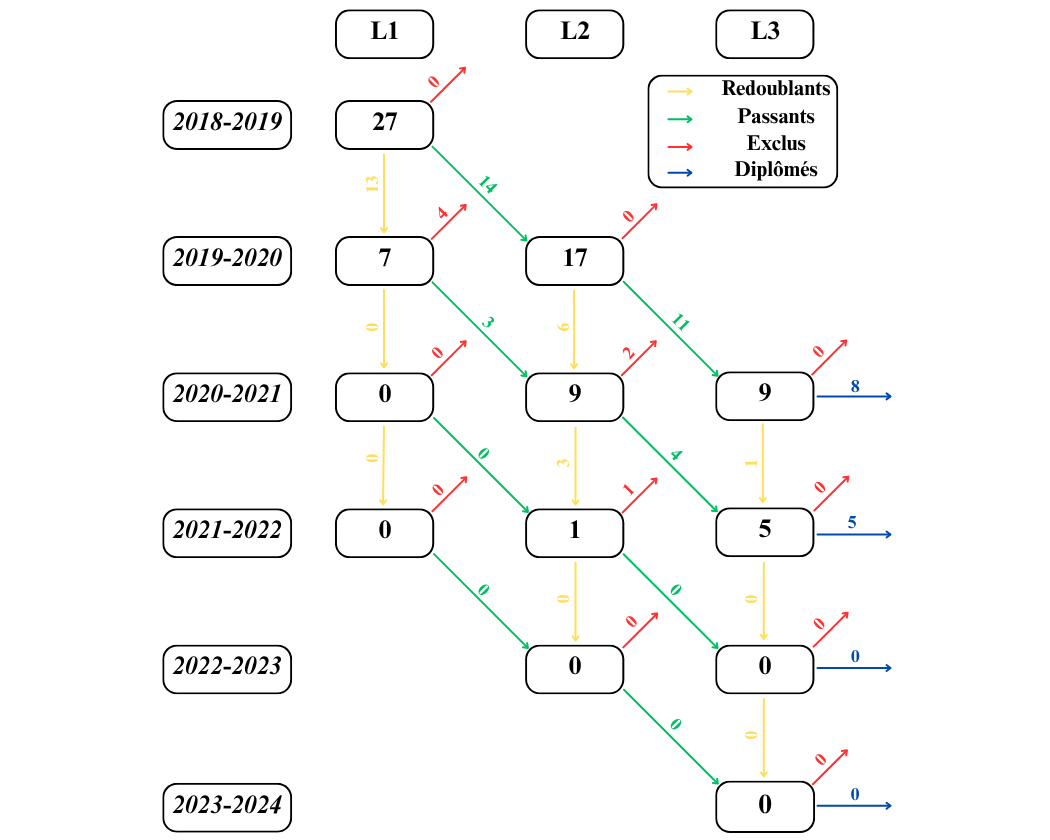
\includegraphics[width=1\textwidth]{figure/S2A_2018.png}
    \label{fig:cohorte_s2a_2018}
\end{figure}

La figure \ref{fig:cohorte_s2a_2018} illustre le suivi de la cohorte 2018 de la série S2A.
\begin{itemize}
    \item Après 3 ans (en 2020-2021), sur les 27 étudiants initiaux en L1 en 2018-2019, 8 ont obtenu leur diplôme, soit un taux de diplomation d'environ 29.63\%.
    \item Après 4 ans (en 2021-2022), 5 étudiants supplémentaires ont été diplômés, portant le total à 13 diplômés, soit un taux cumulé d'environ 48.15\%.
    \item Après 5 ans (en 2022-2023), aucun étudiant supplémentaire n'a été diplômé, le total restant à 13 diplômés, soit un taux cumulé d'environ 48.15\%.
    \item Après 6 ans (en 2023-2024), aucun étudiant supplémentaire n'a été diplômé, le total restant à 13 diplômés, soit un taux cumulé d'environ 48.15\%.
\end{itemize}

\newpage
\subsubsection{cohorte 2018(S1A)}

\begin{figure}[ht]
    \centering
    \caption{Graphe suivi de la cohorte 2018 (S1A)}
    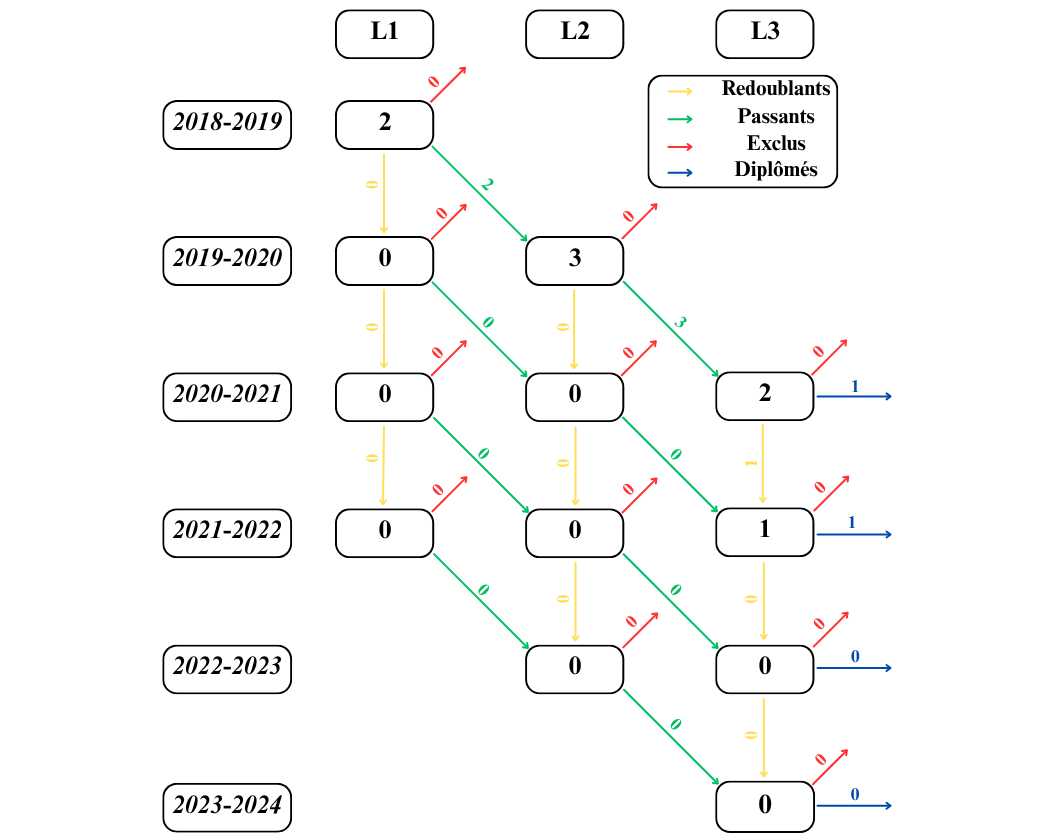
\includegraphics[width=1\textwidth]{figure/S1A_2018.png}
    \label{fig:cohorte_s1a_2018}
\end{figure}

La figure \ref{fig:cohorte_s1a_2018} montre le suivi de la cohorte 2018 de la série S1A.
\begin{itemize}
    \item Après 3 ans (en 2020-2021), sur les 2 étudiants initiaux en L1 en 2018-2019, 1 a obtenu son diplôme, soit un taux de diplomation de 50\%.
    \item Après 4 ans (en 2021-2022), 1 étudiant supplémentaire a été diplômé, portant le total à 2 diplômés, soit un taux cumulé de 100\%.
    \item Après 5 ans (en 2022-2023), aucun étudiant supplémentaire n'a été diplômé.
    \item Après 6 ans (en 2023-2024), aucun étudiant supplémentaire n'a été diplômé.
\end{itemize}

\newpage
\subsection{Série de reference pour les séries Arabes et Franco-Arabes}

\subsubsection{cohorte 2018(L'1)}

\begin{figure}[ht]
    \centering
    \caption{Graphe suivi de la cohorte 2018 (L'1)}
    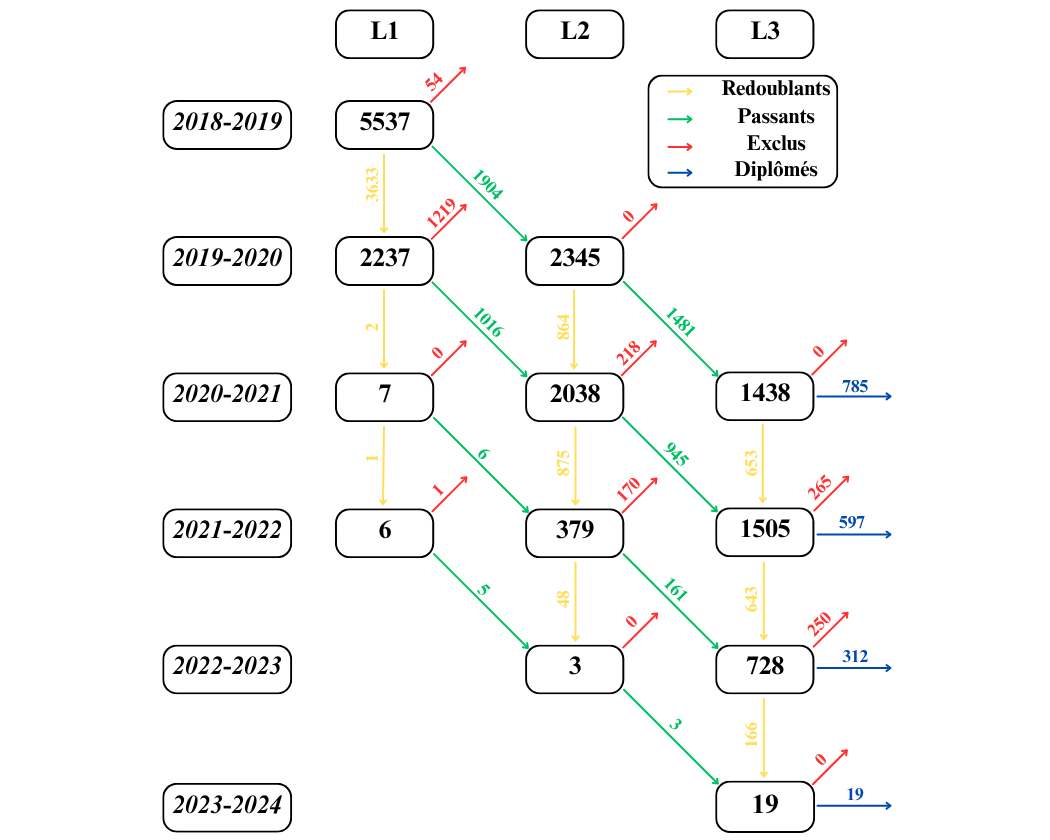
\includegraphics[width=1\textwidth]{figure/L1_2018.png}
    \label{fig:cohorte_l1_2018}
\end{figure}

La figure \ref{fig:cohorte_l1_2018} présente le suivi de la cohorte 2018 de la série L1.
\begin{itemize}
    \item Après 3 ans (en 2020-2021), sur les 5537 étudiants initiaux en L1 en 2018-2019, 785 ont obtenu leur diplôme, soit un taux de diplomation d'environ 14.18\%.
    \item Après 4 ans (en 2021-2022), 597 étudiants supplémentaires ont été diplômés, portant le total à 1382 diplômés, soit un taux cumulé d'environ 24.96\%.
    \item Après 5 ans (en 2022-2023), 312 étudiants supplémentaires ont été diplômés, portant le total à 1694 diplômés, soit un taux cumulé d'environ 30.59\%.
    \item Après 6 ans (en 2023-2024), 19 étudiants supplémentaires ont été diplômés, portant le total à 1713 diplômés, soit un taux cumulé d'environ 30.94\%.
\end{itemize}

\newpage
\subsubsection{cohorte 2018(S2)}

\begin{figure}[ht]
    \centering
    \caption{Graphe suivi de la cohorte 2018 (S2)}
    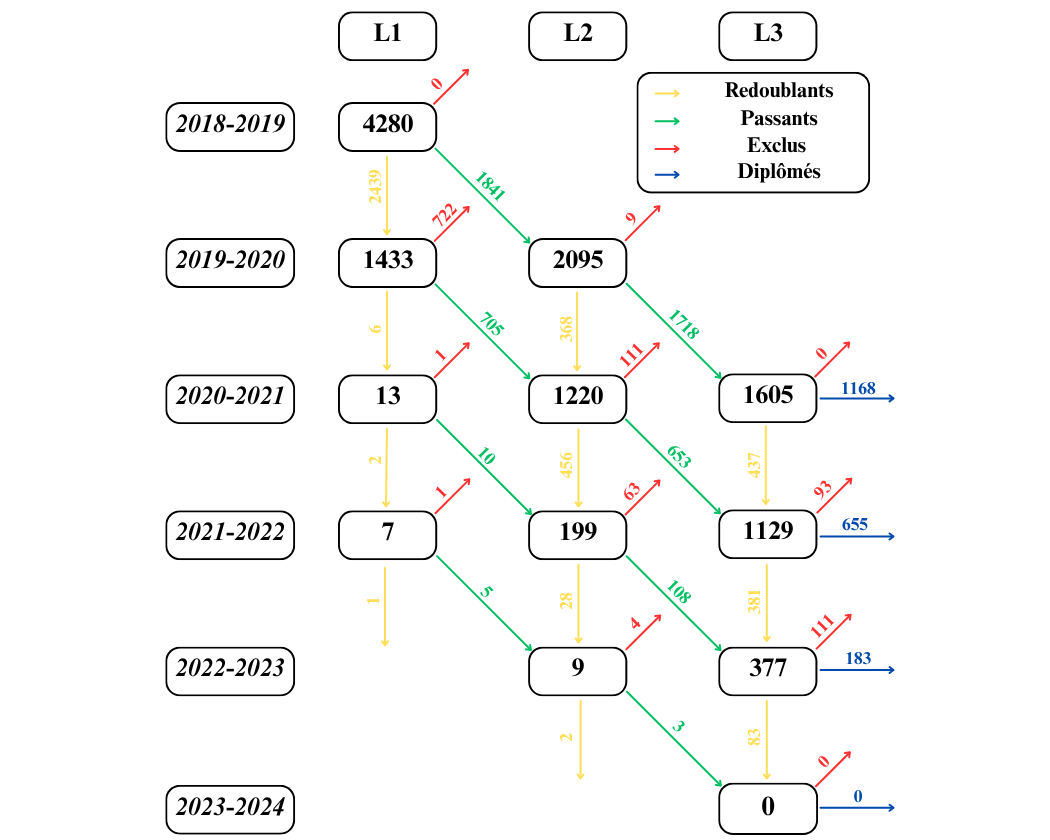
\includegraphics[width=1\textwidth]{figure/S2_2018.png}
    \label{fig:cohorte_s2_2018}
\end{figure}

La figure \ref{fig:cohorte_s2_2018} illustre le suivi de la cohorte 2018 de la série S2.
\begin{itemize}
    \item Après 3 ans (en 2020-2021), sur les 4280 étudiants initiaux en L1 en 2018-2019, 1168 ont obtenu leur diplôme, soit un taux de diplomation d'environ 27.29\%.
    \item Après 4 ans (en 2021-2022), 655 étudiants supplémentaires ont été diplômés, portant le total à 1823 diplômés, soit un taux cumulé d'environ 42.59\%.
    \item Après 5 ans (en 2022-2023), 183 étudiants supplémentaires ont été diplômés, portant le total à 2006 diplômés, soit un taux cumulé d'environ 46.87\%.
    \item Après 6 ans (en 2023-2024), aucun étudiant supplémentaire n'a été diplômé, le total restant à 2006 diplômés, soit un taux cumulé d'environ 46.87\%.
\end{itemize}

\newpage
\subsubsection{cohorte 2018(S1)}

\begin{figure}[ht]
    \centering
    \caption{Graphe suivi de la cohorte 2018 (S1)}
    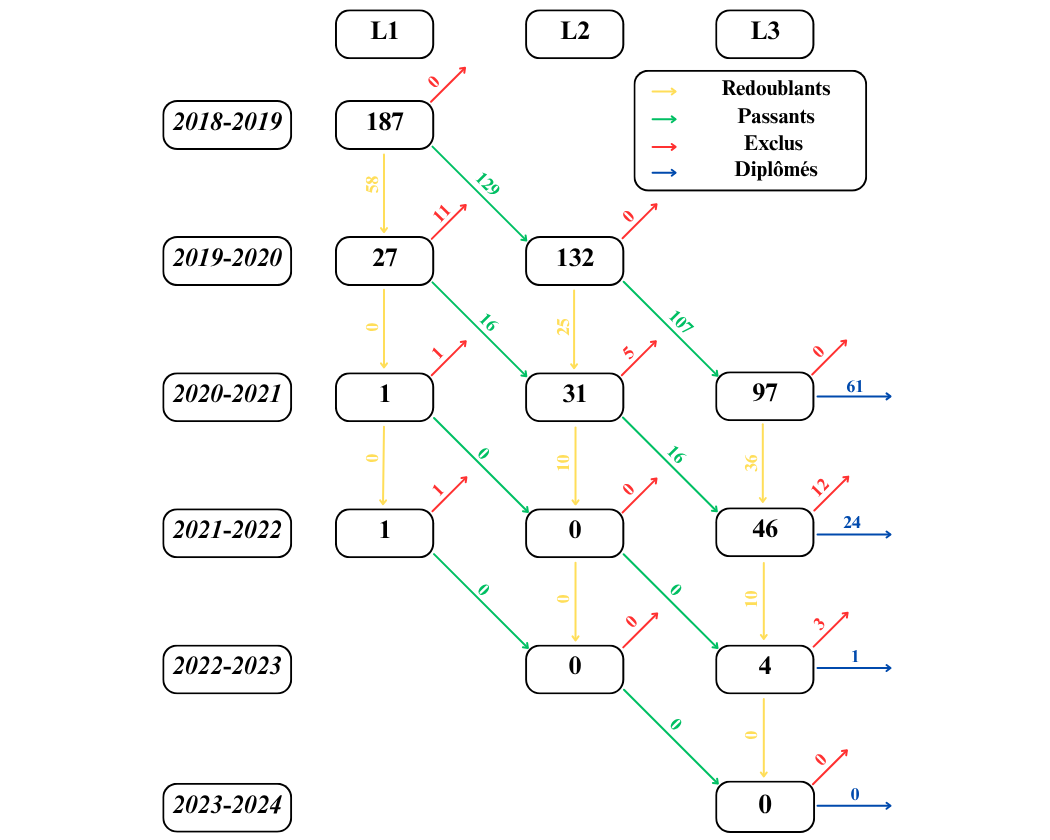
\includegraphics[width=1\textwidth]{figure/S1_2018.png}
    \label{fig:cohorte_s1_2018}
\end{figure}

La figure \ref{fig:cohorte_s1_2018} montre le suivi de la cohorte 2018 de la série S1.
\begin{itemize}
    \item Après 3 ans (en 2020-2021), sur les 187 étudiants initiaux en L1 en 2018-2019, 61 ont obtenu leur diplôme, soit un taux de diplomation d'environ 32.62\%.
    \item Après 4 ans (en 2021-2022), 24 étudiants supplémentaires ont été diplômés, portant le total à 85 diplômés, soit un taux cumulé d'environ 45.45\%.
    \item Après 5 ans (en 2022-2023), 1 étudiant supplémentaire a été diplômé, portant le total à 86 diplômés, soit un taux cumulé d'environ 45.99\%.
    \item Après 6 ans (en 2023-2024), aucun étudiant supplémentaire n'a été diplômé, le total restant à 86 diplômés, soit un taux cumulé d'environ 45.99\%.
\end{itemize}

\newpage
\subsection{Série STEG et G}

\subsubsection{cohorte 2018(G)}

\begin{figure}[ht]
    \centering
    \caption{Graphe suivi de la cohorte 2018 (G)}
    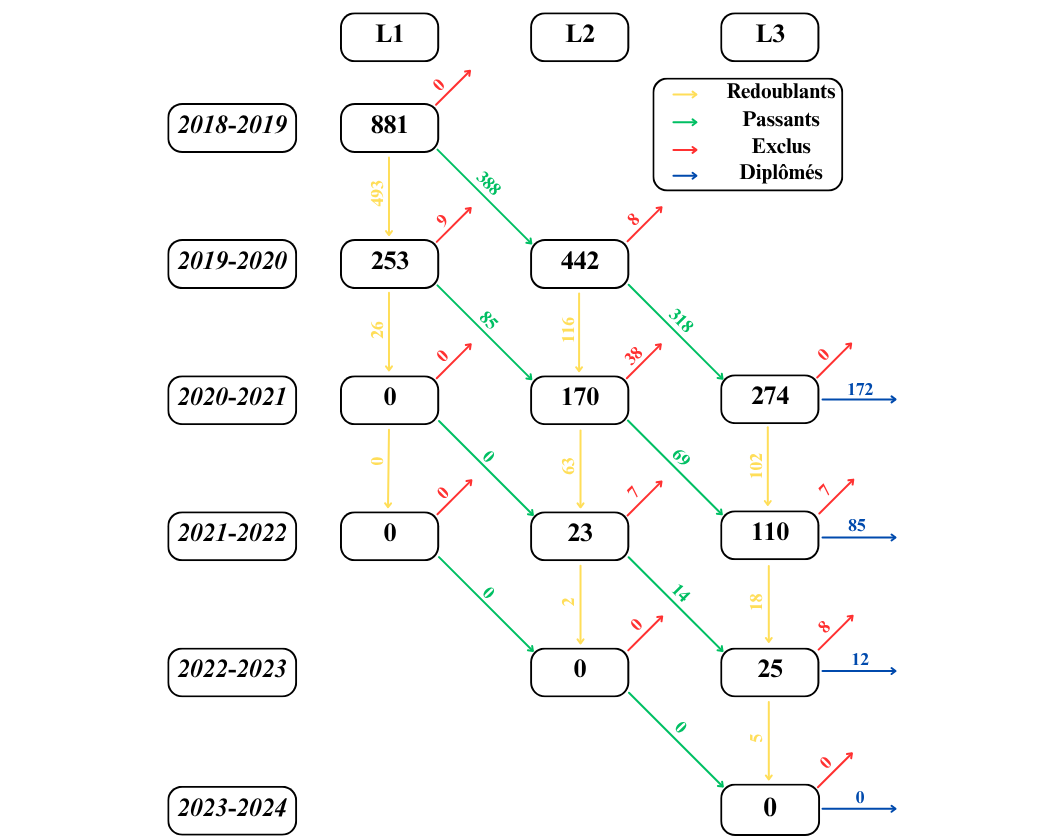
\includegraphics[width=1\textwidth]{figure/G_2018.png}
    \label{fig:cohorte_g_2018}
\end{figure}

La figure \ref{fig:cohorte_g_2018} illustre le suivi de la cohorte 2018 de la série G.
\begin{itemize}
    \item Après 3 ans (en 2020-2021), sur les 630 étudiants initiaux en L1 en 2018-2019, 126 ont obtenu leur diplôme, soit un taux de diplomation d'environ 20\%.
    \item Après 4 ans (en 2021-2022), 52 étudiants supplémentaires ont été diplômés, portant le total à 178 diplômés, soit un taux cumulé d'environ 28.25\%.
    \item Après 5 ans (en 2022-2023), 11 étudiants supplémentaires ont été diplômés, portant le total à 189 diplômés, soit un taux cumulé d'environ 30\%.
    \item Après 6 ans (en 2023-2024), aucun étudiant supplémentaire n'a été diplômé, le total restant à 189 diplômés, soit un taux cumulé d'environ 30\%.
\end{itemize}

\newpage
\subsubsection{cohorte 2019(STEG)}

\begin{figure}[ht]
    \centering
    \caption{Graphe suivi de la cohorte 2019 (STEG)}
    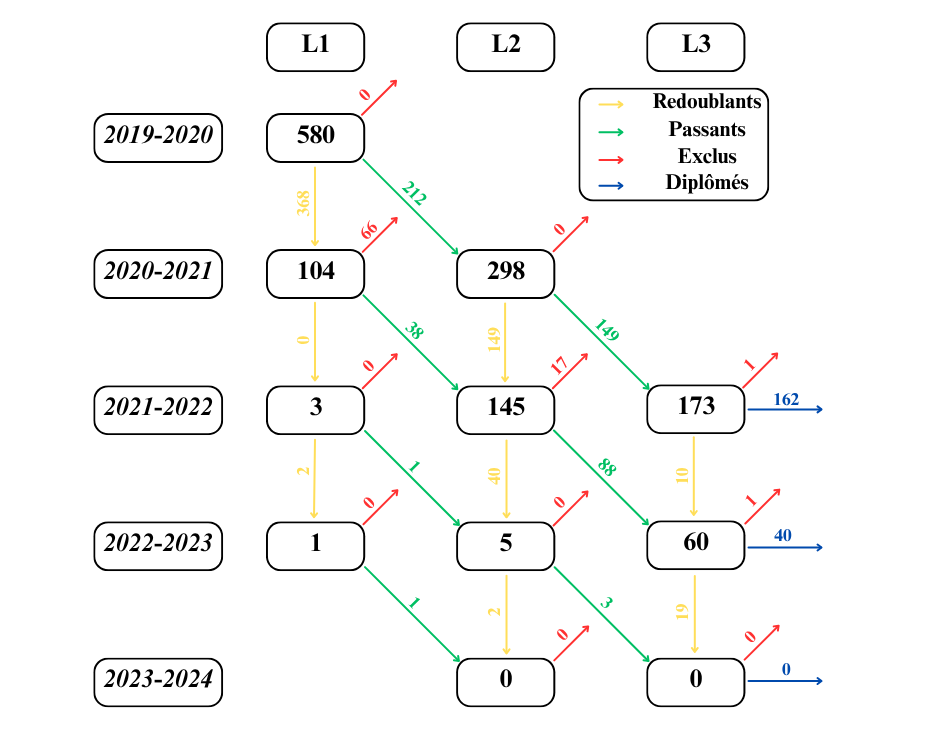
\includegraphics[width=1\textwidth]{figure/STEG_2019.png}
    \label{fig:cohorte_steg_2019}
\end{figure}

La figure \ref{fig:cohorte_steg_2019} présente le suivi de la cohorte 2019 de la série STEG.
\begin{itemize}
    \item Après 3 ans (en 2021-2022), sur les 580 étudiants initiaux en L1 en 2019-2020, 162 ont obtenu leur diplôme, soit un taux de diplomation d'environ 27.93\%.
    \item Après 4 ans (en 2022-2023), 40 étudiants supplémentaires ont été diplômés, portant le total à 202 diplômés, soit un taux cumulé d'environ 34.83\%.
    \item Après 5 ans (en 2023-2024), aucun étudiant supplémentaire n'a été diplômé, le total restant à 202 diplômés, soit un taux cumulé d'environ 34.83\%.
\end{itemize}

\newpage
\section{Analyse des performances académiques}

\subsection{Comparaison des séries LA, LAR et L1 (Cohorte 2018)}

\begin{table}[htbp]
\centering
\caption{Comparaison détaillée des séries LA, LAR et L1 (Cohorte 2018)}
\begin{tabular}{l|c|c|c|c|c|c|}
\cline{2-7}
& \multicolumn{2}{c|}{\textbf{LA}} & \multicolumn{2}{c|}{\textbf{LAR}} & \multicolumn{2}{c|}{\textbf{L1}} \\
\hline
\textbf{Effectif Initial (L1)} & \multicolumn{2}{c|}{131} & \multicolumn{2}{c|}{465} & \multicolumn{2}{c|}{5537} \\
\hline
\textbf{Critère} & \textbf{Diplômés} & \textbf{Taux} & \textbf{Diplômés} & \textbf{Taux} & \textbf{Diplômés} & \textbf{Taux} \\
\hline
\textbf{Après 3 ans} & 29 & 22.14\% & 147 & 31.61\% & 785 & 14.18\% \\
\textbf{Après 4 ans} & 49 & 59.54\% & 49 & 42.15\% & 597 & 24.96\% \\
\textbf{Après 5 ans} & 5 & 63.36\% & 17 & 45.81\% & 312 & 30.59\% \\
\textbf{Après 6 ans} & 0 & 63.36\% & 0 & 45.81\% & 19 & 30.94\% \\
\hline
\end{tabular}
\end{table}

Les séries arabes (LA et LAR) semblent avoir des taux de diplomation plus élevés que la série L1 après 3 ans. 
Notamment, la série LAR présente le meilleur taux de diplomation initial. Sur le long terme (4 à 6 ans), la série LA montre une meilleure persévérance avec un taux cumulé plus élevé que LAR, et toutes deux surpassent significativement la série L1 en termes de taux de diplomation.
Cela pourrait suggérer que les étudiants des filières franco-arabes et arabes sont potentiellement mieux préparés ou trouvent une meilleure adéquation avec les cursus universitaires qui leur sont proposés. 
Cependant, il est important de noter que l'effectif initial de la série L1 est considérablement plus élevé, ce qui peut influencer les pourcentages.

\subsection{Comparaison des séries S2A et S2 (Cohorte 2018)}

\begin{table}[htbp]
\centering
\caption{Comparaison détaillée des séries S2A et S2 (Cohorte 2018)}
\begin{tabular}{l|c|c|c|c|}
\cline{2-5}
& \multicolumn{2}{c|}{\textbf{S2A}} & \multicolumn{2}{c|}{\textbf{S2}} \\
\hline
\textbf{Effectif Initial (L1)} & \multicolumn{2}{c|}{27} & \multicolumn{2}{c|}{4280} \\
\hline
\textbf{Critère} & \textbf{Diplômés} & \textbf{Taux} & \textbf{Diplômés} & \textbf{Taux} \\
\hline
\textbf{Après 3 ans} & 8 & 29.63\% & 1168 & 27.29\% \\
\textbf{Après 4 ans} & 5 & 48.15\% & 655 & 42.59\% \\
\textbf{Après 5 ans} & 0 & 48.15\% & 183 & 46.87\% \\
\textbf{Après 6 ans} & 0 & 48.15\% & 0 & 46.87\% \\
\hline
\end{tabular}
\end{table}

Les performances entre S2A et S2 sont assez similaires. La S2A a un léger avantage sur le taux de diplomation après 3 ans (29.63\% contre 27.29\% pour S2) et après 4 ans (48.15\% contre 42.59\% pour S2). 
Le taux final cumulé est également légèrement supérieur pour la S2A. 
Ces résultats suggèrent que les bacheliers des séries scientifiques arabes s'en sortent aussi bien, voire un peu mieux, que leurs homologues des séries scientifiques générales en termes de réussite universitaire, bien que la S2A ait un effectif beaucoup plus petit.

\subsection{Comparaison des séries S1A et S1 (Cohorte 2018)}

\begin{table}[htbp]
\centering
\caption{Comparaison détaillée des séries S1A et S1 (Cohorte 2018)}
\begin{tabular}{l|c|c|c|c|} 
\cline{2-5} 
& \multicolumn{2}{c|}{\textbf{S1A}} & \multicolumn{2}{c|}{\textbf{S1}} \\
\hline
\textbf{Effectif Initial (L1)} & \multicolumn{2}{c|}{2} & \multicolumn{2}{c|}{187} \\
\hline
\textbf{Critère} & \textbf{Diplômés} & \textbf{Taux} & \textbf{Diplômés} & \textbf{Taux} \\
\hline
\textbf{Après 3 ans} & 1 & 50\% & 61 & 32.62\% \\
\textbf{Après 4 ans} & 1 & 100\% & 24 & 45.45\% \\
\textbf{Après 5 ans} & 0 & 100\% & 1 & 45.99\% \\
\textbf{Après 6 ans} & 0 & 100\% & 0 & 45.99\% \\
\hline
\end{tabular}
\end{table}

La série S1A, bien que basée sur un très petit effectif initial de 2 étudiants, affiche un taux de diplomation exceptionnel de 100\% après 4 ans. 
La série S1, avec un effectif plus représentatif, montre un taux de diplomation respectable de 32.62\% après 3 ans et atteint près de 46\% après 4 ans. 
Il est difficile de tirer des conclusions solides sur S1A en raison de son très faible nombre d'étudiants, mais la S1 démontre une performance solide en termes de diplomation par rapport à d'autres séries généralistes.

\subsection{Comparaison des séries G (Cohorte 2018) et STEG (Cohorte 2019)}

\begin{table}[htbp]
\centering
\caption{Comparaison détaillée des séries G (Cohorte 2018) et STEG (Cohorte 2019)}
\begin{tabular}{l|c|c|c|c|}
\cline{2-5}
& \multicolumn{2}{c|}{\textbf{G (Cohorte 2018)}} & \multicolumn{2}{c|}{\textbf{STEG (Cohorte 2019)}} \\
\hline
\textbf{Effectif Initial (L1)} & \multicolumn{2}{c|}{630} & \multicolumn{2}{c|}{580} \\
\hline
\textbf{Critère} & \textbf{Diplômés} & \textbf{Taux} & \textbf{Diplômés} & \textbf{Taux} \\
\hline
\textbf{Après 3 ans} & 126 & 20\% & 162 & 27.93\% \\
\textbf{Après 4 ans} & 52 & 28.25\% & 40 & 34.83\% \\
\textbf{Après 5 ans} & 11 & 30\% & 0 & 34.83\% \\
\textbf{Après 6 ans} & 0 & 30\% & N/A & N/A \\
\hline
\end{tabular}
\end{table}

La comparaison entre la série G (cohorte 2018) et la nouvelle série STEG (cohorte 2019) est particulièrement pertinente étant donné la réforme. Les données montrent que la série STEG présente un taux de diplomation après 3 ans nettement supérieur (27.93\%) à celui de la série G (20\%). De même, le taux cumulé après 4 ans pour STEG (34.83\%) est plus élevé que celui de la série G sur la même période (28.25\%). 
Ces chiffres suggèrent que la réforme de transformation de la série G en STEG a eu un impact positif sur les performances académiques des étudiants, potentiellement en raison d'une meilleure adéquation des programmes aux exigences de l'enseignement supérieur ou une meilleure préparation des étudiants.
La réforme visait à arrimer ce Baccalauréat aux exigences de la réforme de la Formation professionnelle et technique (FPT) et de l'Enseignement supérieur, avec un objectif de recentrer les contenus des programmes pour augmenter les chances de réussite des apprenants. La série G a été transformée en série technologique (sciences et technologies de l'économie et de la gestion: STEG).
Les données présentées semblent valider cette démarche.

\section{Conclusion}

L'étude du parcours universitaire des bacheliers à l'UCAD, suite aux réformes du baccalauréat, révèle des dynamiques d'orientation marquées et, pour la plupart, cohérentes avec les objectifs des réformes.

Concernant la série STEG, la transition depuis l'ancienne série G s'est traduite par une orientation massive des étudiants vers la Faculté des Sciences Économiques et de Gestion (FASEG) et, dans une moindre mesure, vers l'École Supérieure Polytechnique (ESP), notamment dans les départements de gestion et d'entrepreneuriat. 
Cette concentration des effectifs confirme que la série STEG a su remplir son rôle de passerelle vers les filières universitaires d'économie et de gestion, assurant une continuité fonctionnelle avec la série qu'elle a remplacée.

Pour les séries arabes et franco-arabes, la Faculté des Lettres et Sciences Humaines (FLSH) et son département d'Arabe sont clairement les destinations privilégiées pour les bacheliers LA et surtout LAR. La série LAR, avec son volume d'inscriptions plus important, s'est imposée comme la voie royale pour les études arabes à l'UCAD, validant l'effort de structuration de ces filières. 
Quant à la série S2A, elle oriente principalement ses étudiants vers la Faculté des Sciences et Technologies (FST), avec des ouvertures significatives vers la FASEG et la Faculté de Médecine, de Pharmacie et d'Odontologie (FMPO), reflétant la polyvalence et les débouchés variés de cette série scientifique appliquée. 
En revanche, la série S1A demeure anecdotique en termes d'inscriptions universitaires, confirmant son caractère marginal dans le paysage éducatif sénégalais.

Globalement, les données sur l'orientation à l'UCAD suggèrent que les réformes du baccalauréat ont réussi à guider les étudiants vers des filières universitaires en adéquation avec leur spécialisation au secondaire. 
La question de la réussite et de la progression académique de ces cohortes au sein de l'université reste cependant ouverte, et nécessiterait une analyse de suivi de cohorte sur plusieurs années pour évaluer pleinement l'impact des réformes sur la persévérance et le succès des étudiants une fois entrés dans l'enseignement supérieur.